% Options for packages loaded elsewhere
\PassOptionsToPackage{unicode}{hyperref}
\PassOptionsToPackage{hyphens}{url}
%
\documentclass[
  11pt,
  a4paper,
]{scrbook}

\usepackage{amsmath,amssymb}
\usepackage{setspace}
\usepackage{iftex}
\ifPDFTeX
  \usepackage[T1]{fontenc}
  \usepackage[utf8]{inputenc}
  \usepackage{textcomp} % provide euro and other symbols
\else % if luatex or xetex
  \usepackage{unicode-math}
  \defaultfontfeatures{Scale=MatchLowercase}
  \defaultfontfeatures[\rmfamily]{Ligatures=TeX,Scale=1}
\fi
\usepackage{lmodern}
\ifPDFTeX\else  
    % xetex/luatex font selection
\fi
% Use upquote if available, for straight quotes in verbatim environments
\IfFileExists{upquote.sty}{\usepackage{upquote}}{}
\IfFileExists{microtype.sty}{% use microtype if available
  \usepackage[]{microtype}
  \UseMicrotypeSet[protrusion]{basicmath} % disable protrusion for tt fonts
}{}
\makeatletter
\@ifundefined{KOMAClassName}{% if non-KOMA class
  \IfFileExists{parskip.sty}{%
    \usepackage{parskip}
  }{% else
    \setlength{\parindent}{0pt}
    \setlength{\parskip}{6pt plus 2pt minus 1pt}}
}{% if KOMA class
  \KOMAoptions{parskip=half}}
\makeatother
\usepackage{xcolor}
\usepackage[textheight=9in,,textwidth=6.5in,,top=1in,,headheight=14pt,,headsep=25pt,,footskip=30pt]{geometry}
\ifLuaTeX
  \usepackage{luacolor}
  \usepackage[soul]{lua-ul}
\else
  \usepackage{soul}
  
\fi
\setlength{\emergencystretch}{3em} % prevent overfull lines
\setcounter{secnumdepth}{2}
% Make \paragraph and \subparagraph free-standing
\makeatletter
\ifx\paragraph\undefined\else
  \let\oldparagraph\paragraph
  \renewcommand{\paragraph}{
    \@ifstar
      \xxxParagraphStar
      \xxxParagraphNoStar
  }
  \newcommand{\xxxParagraphStar}[1]{\oldparagraph*{#1}\mbox{}}
  \newcommand{\xxxParagraphNoStar}[1]{\oldparagraph{#1}\mbox{}}
\fi
\ifx\subparagraph\undefined\else
  \let\oldsubparagraph\subparagraph
  \renewcommand{\subparagraph}{
    \@ifstar
      \xxxSubParagraphStar
      \xxxSubParagraphNoStar
  }
  \newcommand{\xxxSubParagraphStar}[1]{\oldsubparagraph*{#1}\mbox{}}
  \newcommand{\xxxSubParagraphNoStar}[1]{\oldsubparagraph{#1}\mbox{}}
\fi
\makeatother


\providecommand{\tightlist}{%
  \setlength{\itemsep}{0pt}\setlength{\parskip}{0pt}}\usepackage{longtable,booktabs,array}
\usepackage{calc} % for calculating minipage widths
% Correct order of tables after \paragraph or \subparagraph
\usepackage{etoolbox}
\makeatletter
\patchcmd\longtable{\par}{\if@noskipsec\mbox{}\fi\par}{}{}
\makeatother
% Allow footnotes in longtable head/foot
\IfFileExists{footnotehyper.sty}{\usepackage{footnotehyper}}{\usepackage{footnote}}
\makesavenoteenv{longtable}
\usepackage{graphicx}
\makeatletter
\newsavebox\pandoc@box
\newcommand*\pandocbounded[1]{% scales image to fit in text height/width
  \sbox\pandoc@box{#1}%
  \Gscale@div\@tempa{\textheight}{\dimexpr\ht\pandoc@box+\dp\pandoc@box\relax}%
  \Gscale@div\@tempb{\linewidth}{\wd\pandoc@box}%
  \ifdim\@tempb\p@<\@tempa\p@\let\@tempa\@tempb\fi% select the smaller of both
  \ifdim\@tempa\p@<\p@\scalebox{\@tempa}{\usebox\pandoc@box}%
  \else\usebox{\pandoc@box}%
  \fi%
}
% Set default figure placement to htbp
\def\fps@figure{htbp}
\makeatother

% Palatino font:
\usepackage[T1]{fontenc}
\usepackage[utf8]{inputenc}


% Add new fonts 
\usepackage{newpxtext}
\usepackage{newpxmath}


% % Palatino and math font to match
% \usepackage{palatino}
% \usepackage{mathpazo}

\usepackage{upquote}

% front page
\usepackage[colorlinks]{hyperref} % for text color on title
\usepackage{titling} % makes \thetitle etc available...
\usepackage{lipsum}
\usepackage{tikz}
\tikzstyle{bag} = [align=center] % allows new lines in text below
\AtBeginDocument{\thispagestyle{empty}
\definecolor{titlecolor}{HTML}{1C2404}
\begin{tikzpicture}[remember picture,overlay]
\draw (current page.center) node[inner sep=0, opacity=0.5] {\resizebox{!}{350mm}{\includegraphics{highres_banner.pdf}}};
\draw (current page.center) node[inner sep=0, opacity=0.5] {\resizebox{!}{100mm}{
\includegraphics{ausegl_sort.pdf}}};
% \draw (current page.center) node[bag] {  
        \draw (17, 1.7) node[bag, align=right, anchor=north east] {  
    % \mytitlefont 
    \color{titlecolor} \Large \textbf{Thesis} \\ 
    \\ 
    % \mytitlefont 
    \color{titlecolor} \Huge \textbf{\thetitle} \\ 
    \\ 
    % \mytitlefont
    \color{titlecolor} \huge \theauthor \\
    \\
    % \mytitlefont 
    \color{titlecolor} \Large \thedate 
    };
\end{tikzpicture}
\clearpage}

% back side
\AtEndDocument{\clearpage\thispagestyle{empty}
\begin{tikzpicture}[remember picture,overlay]
\draw (current page.center) node[inner sep=0, opacity=0.5] {\resizebox{!}{350mm}{\includegraphics{highres_banner.pdf}}};
% \draw (current page.center) node[bag] {  
    \draw (17, 1.7) node[bag, align=right, anchor=north east] {  
        % \mytitlefont 
        \color{titlecolor} \large Bioinformatics Research Centre \\ 
        % \mytitlefont 
        \color{titlecolor} \large Department of Molecular Biology and Genetics \\ 
        % \mytitlefont 
        \color{titlecolor} \large Aarhus University \\
        % \mytitlefont 
        \color{titlecolor} \large Universitetsbyen 81 \\
        % \mytitlefont 
        \color{titlecolor} \large 8000 Aarhus C \\
        % \mytitlefont 
        \color{titlecolor} \large Denmark
        };

\end{tikzpicture}}


% % picture (AU logo in title page)
% \usepackage{titlepic}
% % \usepackage{graphicx}
% \titlepic{\resizebox{!}{50mm}{
\includegraphics[width=\textwidth]{ausegl_sort.pdf}}}



% \pagestyle{plain} % no running header

\usepackage[many]{tcolorbox}
\definecolor{quotegray}{HTML}{505050}
\newtcolorbox{myquote}{%
    enhanced jigsaw, 
    breakable,      % allow page breaks
    frame hidden,   % hide the default frame
    left=1cm,       % left margin
    right=1cm,      % right margin
    colback=white,
    fontupper=\color{quotegray},
    overlay={%
        \node [scale=4,
            text=lightgray,
            inner sep=0pt,] at ([xshift=0.5cm,yshift=-0.7cm]frame.north west){``}; 
        \node [scale=4,
            text=lightgray,
            inner sep=0pt,] at ([xshift=-0.5cm]frame.south east){''};  
            },
        % paragraph skips obeyed within tcolorbox
                parbox=false,
}
% redefine the 'quote' environment to use this 'myquote' environment
\renewenvironment{quote}{\begin{myquote}}{\end{myquote}}

% add a dummy abstract environment that is defined in quarto manuscript 
% but not in the quarto book that we run first to give it a slot in the 
% side bar
\ifcsmacro{abstract}{}{
  \let\endmyenvironment\undefined%
  \newenvironment{abstract}{\chapter*{Abstract}}{}
}

% \usepackage{framed} % not sure i need this anymore

% \usepackage[T1]{fontenc}
% \usepackage{inconsolata}

% % I have to only define Shaded if it is already defined.
% % The reason is that pandoc does not define the macro if there are not code blocks in the a markdown file.
% \ifx \@Shaded \@empty

% \renewcommand{\KeywordTok}[1]{\textcolor[rgb]{0, 0, 0}{\textbf{{#1}}}} % def and or not reg
% \renewcommand{\BuiltInTok}[1]{\textcolor[rgb]{0.373, 0.298, 0.580}{\textbf{{#1}}}} % print open 
% \renewcommand{\VariableTok}[1]{\textcolor[rgb]{0.141, 0.392, 0.824}{\textbf{{#1}}}}
% \renewcommand{\OperatorTok}[1]{\textcolor[rgb]{0, 0, 0}{{#1}}} % def and or not reg
% \renewcommand{\DataTypeTok}[1]{\textcolor[rgb]{1.0,0.13,0.00}{{#1}}}
% \renewcommand{\DecValTok}[1]{\textcolor[rgb]{0.655, 0.498, 0.161}{{#1}}}
% \renewcommand{\BaseNTok}[1]{\textcolor[rgb]{0.259, 0.592, 0.596}{{#1}}}
% \renewcommand{\FloatTok}[1]{\textcolor[rgb]{0.655, 0.498, 0.161}{{#1}}}
% \renewcommand{\CharTok}[1]{\textcolor[rgb]{0.678,0.141,0.098}{{#1}}}
% \renewcommand{\StringTok}[1]{\textcolor[rgb]{0.678,0.141,0.098}{{#1}}}
% \renewcommand{\CommentTok}[1]{\textcolor[rgb]{0.135, 0.134, 0.133}{{#1}}}
% \renewcommand{\OtherTok}[1]{\textcolor[rgb]{0.00,0.44,0.13}{{#1}}}
% \renewcommand{\AlertTok}[1]{\textcolor[rgb]{1.00,0.00,0.00}{\textbf{{#1}}}}
% \renewcommand{\FunctionTok}[1]{\textcolor[rgb]{0.549, 0.102, 0.063}{\textbf{{#1}}}}  % function name
% \renewcommand{\RegionMarkerTok}[1]{{#1}}
% \renewcommand{\ErrorTok}[1]{\textcolor[rgb]{1.00,0.00,0.00}{\textbf{{#1}}}}
% \renewcommand{\NormalTok}[1]{\textcolor[rgb]{0, 0, 0}{{#1}}}


% \else
%   % no code blocks with markup...
% \fi



\usepackage{etoolbox}
\makeatletter
\g@addto@macro{\appendix}{%
  \patchcmd{\@@makechapterhead}% <cmd>
    {\endgraf\nobreak\vskip.5\baselineskip}% <search>
    {\hspace*{-.5em}:\space}% <replace>
    {}{}% <success><failure>
  \patchcmd{\@chapter}% <cmd>
    {\addchaptertocentry{\thechapter}}% <search>
    {\addchaptertocentry{Appendix~\thechapter:}}% <replace>
    {}{}% <success><failure>
  \addtocontents{toc}{%
    \protect\patchcmd{\protect\l@chapter}% <cmd>
      {1.5em}% <search>
      {6.5em}% <replace>
      {}{}}% <success><failure>
}
\renewcommand{\autodot}{}% Remove all end-of-counter dots
\makeatother


% restart chapter numbers in each part
\makeatletter
\@addtoreset{chapter}{part}
\makeatother


% \usepackage{chngcntr}
% \counterwithin*{subsubsection}{chapter}
% \counterwithout*{subsubsection}{section}
% \counterwithout*{subsubsection}{subsection}

% %  % KMT only use subsubsection number (this increments though the book 
% %  % when we supress numbering with  {.unnumbered} after each header except Exerisices
% \renewcommand\thesubsubsection{\arabic{section}}
% \renewcommand\thesubsubsection{\arabic{subsection}}
% \renewcommand\thesubsubsection{\arabic{chapter}-\arabic{subsubsection}}


\renewcommand*{\chapterformat}{%
\textcolor[rgb]{0.7, 0.7, 0.7}{\thechapter}\autodot\enskip%
}
\renewcommand*{\sectionformat}{%
\textcolor[rgb]{0.7, 0.7, 0.7}{\thesection}\autodot\enskip%
}
\renewcommand*{\subsectionformat}{%
\textcolor[rgb]{0.7, 0.7, 0.7}{\thesubsection}\autodot\enskip%
}
\renewcommand*{\subsubsectionformat}{%
\textcolor[rgb]{0.7, 0.7, 0.7}{\thesubsubsection}\autodot\enskip%
}

% %% from arcxiv.sty:  %%%
\RedeclareSectionCommand[
  beforeskip=-2ex,
  afterskip=1.5ex
]{chapter}

\RedeclareSectionCommand[
  beforeskip=-1.8ex,
  afterskip=0.8ex
]{section}

\RedeclareSectionCommand[
  beforeskip=--1.5ex,
  afterskip=0.5ex
]{subsection}

\RedeclareSectionCommand[
  beforeskip=1.5ex,
  afterskip=-1em
]{subsubsection}

\RedeclareSectionCommand[
  beforeskip=1.5ex,
  afterskip=-1em
]{paragraph}

% \RedeclareSectionCommand[
%   beforeskip=1.5ex plus 0.5ex minus 0.2ex,
%   afterskip=-1em
% ]{subparagraph}


\setkomafont{section}{\normalfont\Large\bfseries\raggedright}
\setkomafont{subsection}{\normalfont\large\bfseries\raggedright}
\setkomafont{subsubsection}{\normalfont\normalsize\bfseries\raggedright}
\setkomafont{paragraph}{\normalfont\normalsize\bfseries}
\setkomafont{subparagraph}{\normalfont\normalsize\bfseries}

\setkomafont{caption}{\small}
\setkomafont{captionlabel}{\bfseries\sffamily}

%% Tables
% \usepackage{floatrow}
% \floatsetup[table]{font=small}
\usepackage{booktabs} % professional-quality tables (arxiv.sty)
\usepackage{caption}
\captionsetup[subfigure]{font=scriptsize,labelfont=scriptsize, position=top}

%%%


% % prevent latex from "floating" the figures
% \usepackage{float}
% \let\origfigure\figure
% \let\endorigfigure\endfigure
% \renewenvironment{figure}[1][2] {
%     \expandafter\origfigure\expandafter[H]
% } {
%     \endorigfigure
% }

\usepackage{xcolor}
% \let\oldtextit\textit 
% \renewcommand\textit[1]{\oldtextit{\color{blue}#1}}
\let\oldemph\emph
\renewcommand\emph[1]{\oldemph{\color{gray}#1}}

\makeatletter
\@ifpackageloaded{caption}{}{\usepackage{caption}}
\AtBeginDocument{%
\ifdefined\contentsname
  \renewcommand*\contentsname{Table of contents}
\else
  \newcommand\contentsname{Table of contents}
\fi
\ifdefined\listfigurename
  \renewcommand*\listfigurename{List of Figures}
\else
  \newcommand\listfigurename{List of Figures}
\fi
\ifdefined\listtablename
  \renewcommand*\listtablename{List of Tables}
\else
  \newcommand\listtablename{List of Tables}
\fi
\ifdefined\figurename
  \renewcommand*\figurename{Figure}
\else
  \newcommand\figurename{Figure}
\fi
\ifdefined\tablename
  \renewcommand*\tablename{Table}
\else
  \newcommand\tablename{Table}
\fi
}
\@ifpackageloaded{float}{}{\usepackage{float}}
\floatstyle{ruled}
\@ifundefined{c@chapter}{\newfloat{codelisting}{h}{lop}}{\newfloat{codelisting}{h}{lop}[chapter]}
\floatname{codelisting}{Listing}
\newcommand*\listoflistings{\listof{codelisting}{List of Listings}}
\makeatother
\makeatletter
\makeatother
\makeatletter
\@ifpackageloaded{caption}{}{\usepackage{caption}}
\@ifpackageloaded{subcaption}{}{\usepackage{subcaption}}
\makeatother

\usepackage[]{natbib}
\bibliographystyle{plainnat}
\usepackage{bookmark}

\IfFileExists{xurl.sty}{\usepackage{xurl}}{} % add URL line breaks if available
\urlstyle{same} % disable monospaced font for URLs
\hypersetup{
  pdftitle={Chromatin Compartments and Selection on X},
  pdfkeywords={Hi-C, Chromatin Compartments, Evolutionary
pressures, Selfish gene drive},
  hidelinks,
  pdfcreator={LaTeX via pandoc}}


\title{Chromatin Compartments and Selection on X}
\usepackage{etoolbox}
\makeatletter
\providecommand{\subtitle}[1]{% add subtitle to \maketitle
  \apptocmd{\@title}{\par {\large #1 \par}}{}{}
}
\makeatother
\subtitle{How Edges of Active Chromatin Align with Selection Regions in
Primates}
\author{Søren Jørgensen}
\date{2024-12-27}

\begin{document}
\frontmatter
\cleardoublepage
\thispagestyle{empty}
{\centering
\hbox{}\vskip 0cm plus 1fill

{%\mytitlefont 
\Huge\bfseries Chromatin Compartments and Selection on X \par}
\vspace{3ex}
{\Large\bfseries How Edges of Active Chromatin Align with Selection
Regions in Primates \par}
\vspace{6ex}

    {\Large\bfseries Søren Jørgensen \par}
    %
%
\vskip 0cm plus 2fill

{\resizebox{!}{50mm}{
\includegraphics[width=\textwidth]{hicausegl.pdf}} \par}
\vskip 0cm plus 2fill

{\bfseries\Large\textit{MSc. Bioinformatics} \par}
\vspace{3ex}

{\bfseries\large 2024-12-27 \par}
\vspace{3ex}

\vspace{12ex}
{\small Submitted in fulfillment of the requirements
of the degree of MSc. Bioinformatics \par}
\pagebreak

\begin{quote}
\raggedright    
Here, the 3D chromatin architecture of the X chromosome in rhesus
macaque (\emph{Macaca mulata}) is investigated in the context of
evolutionary pressures and genetic drivers. We redo Hi-C analyses from a
2019 paper on the latest reference genome (\emph{rheMac10} or
\emph{Mmul\_10}). We compare two Hi-C analysis frameworks,
\emph{HiCExplorer} and \emph{cooler/cooltools} (Open2C), on a subset,
finding Open2C to be most flexible and intuitive. The ICE method
(Iterative Correction and Eigendecomposition) was used to infer
conventional and refined A/B compartments for fibroblast and four stages
of spermatogenesis. We find that 200 kbp transition-zones between
A/B-compartments in both fibroblasts and round spermatids align well
with human selective sweeps where meiotic drive can explain the
selection (ECH-regions), and with hybrid incompatility in baboons (genus
\emph{Papio}). We discuss the biological meaning of these findings,
where conserved chromatin features may help to retain non-advantageous
alleles, hinting to the role of selfish genetic elements in genome
evolution. \par
\raggedleft    
    {- Søren Jørgensen \par}
%    
\end{quote}
}

\renewcommand*\contentsname{Table of contents}
{
\setcounter{tocdepth}{1}
\tableofcontents
}

\setstretch{1.25}
\mainmatter
\chapter{Introduction}\label{introduction}

\section{Reproducible Research and
Quarto}\label{reproducible-research-and-quarto}

\section{Sexual reproduction (spermatogenesis,
meiosis)}\label{sexual-reproduction-spermatogenesis-meiosis}

The production of gametes in a sexually reproducing organism is a highly
complex process that involves numeruous elements. Spermatogenesis, the
process of forming male gametes, involves four stages of differentiation
from a germ cell through \emph{spermatogonia}, \emph{pachytene
spermatocyte}, and \emph{round spermatids} to \emph{spermatozoa}, or
\emph{sperm} \citep{wang_reprogramming_2019}, and it is the very basis
of male reproduction. The specialized cell division of meiosis neatly
handles the pairing, recombination, and segregation of homologous
chromosomes, thereby ensuring proper genetic distribution. Deeply
understanding the steps of molecular steps of reproduction and how our
genetic material is inherited is essential in biology, bringing insight
to areas such as speciation, population diversity, and (male)
infertility.

\section{Selfish genes (and
randomness)}\label{selfish-genes-and-randomness}

The conventional story of meiosis in gametogenesis is one of random
segregation of the sex chromosomes. They split into haploid gametes,
where each chromosome has an equal chance of being passed on to a
gamete. That seems like a fair game, but what if some genes are cheating
the system by making others less viable. A meiotic driver is a selfish
gene element that modulates meiosis and preferentially transmits its own
allele through meiosis, regardless of the downstream fitness effects it
may have (good or bad) on the organism it is part of. This phenomenon
challenges the traditional understanding of selection, extending its
scope beyond the fitness effects on an organism to include selective
pressures at the molecular level. For example, if some genes on the X
chromosome create a disadvantage for gametes that \emph{do not} contain
those genes, making sure the Y chromosome is not as viable as the X,
resulting in a sex imbalance and possibly numerous other downstream
effects. That is exactly what is coined \emph{sex chromosome meiotic
drive} \citep{jaenike_sex_2001}, a result of selfish genetic elements.

Motivated by previous results in the Munch Research group
\citep{munch_group_2024} on hybrid incompatibility and extended common
haplotypes \citep{skov_extraordinary_2023, sorensen_genome_wide_2023}
that could be explained by meiotic drive, we wanted to investigate how
these patterns correlate with chromatin compartments.

\section{Our Organism of Interest, Wang et al., and the
references}\label{our-organism-of-interest-wang-et-al.-and-the-references}

\section{Extended Common Haplotypes Discoverved in
Humans}\label{extended-common-haplotypes-discoverved-in-humans}

\section{Chromatin Conformation}\label{chromatin-conformation}

\section{High-Throughput Chromosome Conformation Capture
(Hi-C)}\label{high-throughput-chromosome-conformation-capture-hi-c}

Our DNA can be divided into different orders of structure. \emph{3C}
focus on identifying the highest orders of organization inside the
nucleus, that is, when the 30 nm thick coil of chromatin fibers folds
into loops, Topologically Associating Domains (TADs), and chromatin
compartments. Here, we narrow our focus on the largest of the
structures, \emph{compartments}, that is known to determine availability
to transcription factors, thus making an \emph{A} compartment
\emph{active}---and the \emph{B} compartment \emph{inactive}. The
introduction of the Hi-C (high-throughput 3C) method
\citep{lieberman_aiden_comprehensive_2009} opened new possibilities for
exploring the three-dimensional organization of the genome.

\subsection{Hi-C Library preparation}\label{hi-c-library-preparation}

\subsection{Hi-C Data Analysis}\label{hi-c-data-analysis}

\subsubsection{Aligning the Hi-C reads}\label{aligning-the-hi-c-reads}

\subsubsection{Identifying and Storing Valid Hi-C
Pairs}\label{identifying-and-storing-valid-hi-c-pairs}

\subsubsection{Interaction Matrices and Quality
Control}\label{interaction-matrices-and-quality-control}

\subsubsection{Calling Compartments
(ICE)}\label{calling-compartments-ice}

\subsubsection{Edges}\label{edges}

\chapter{Methods}\label{methods}

In this project, we formulate two objectives:

\textbf{A}: Reproduce the Hi-C interaction maps and eigendecomposition
from \citep{wang_reprogramming_2019}, with some modifications. We
briefly use \emph{HiCExplorer}, but change the analyses to use the
\emph{Open2C Ecosystem} \citep{open2c} which have a Pyton API as well as
command-line functions, which can be paired very well with Jupyter
Notebooks. The majority of the data analysis was run with a \emph{gwf}
workflow, and the commands that were visually inspected were run in
Jupyter Notebooks.

\textbf{B} Compare with regions of selection that are found in
\emph{human}. Investigate the biological meaning of the results.

All computations were performed on GenomeDK (GDK) {[}ref{]}, an HPC
cluster located on Aarhus Uninversity, and most of the processing of the
data was nested into a \emph{gwf} workflow {[}ref{]}, a workflow manager
developed at GDK. I would like to thank GDK and Aarhus University for
providing computational resources and support that contributed to these
research results.

The whole of this project is carried out with reproducibility in mind,
so an effort (and quite a significant amount of time) has been put into
documenting code and organizing the project for readbility and
transparency through a Quarto project {[}ref{]}. Therefore, all code,
virtual environments and text is made available as a Quarto book,
rendered directly from the GitHub repository with GitHub Pages
{[}ref{]}. To make this possible, the Quarto documentation has been
extensively studied and discussed with \emph{KMT} {[}ref, aknowledge{]}.

\section{Initial Exploration with
HiCExplorer}\label{initial-exploration-with-hicexplorer}

Here moves most of the text about HiCExplorer\ldots{}

For the initial exploration of methods with \emph{HiCExplorer}, the 5
first samples in `fibroblast' were chosen
(Table~\ref{tbl-hic-exploration}).

\small

\begin{longtable}[]{@{}lllll@{}}

\caption{\label{tbl-hic-exploration}The samples chosen for initial data
exploration with HiCExplorer. From NCBI SRA Portal.}

\tabularnewline

\toprule\noalign{}
& Run & Bases & Bytes & source\_name \\
\midrule\noalign{}
\endhead
\bottomrule\noalign{}
\endlastfoot
0 & SRR6502335 & 73201141800 & 31966430779 & fibroblast \\
1 & SRR6502336 & 65119970100 & 24433383054 & fibroblast \\
2 & SRR6502337 & 52769196300 & 23015357755 & fibroblast \\
3 & SRR6502338 & 52378949100 & 22999581685 & fibroblast \\
4 & SRR6502339 & 28885941600 & 10960123150 & fibroblast \\

\end{longtable}

\normalsize

The goal was to replicate some of the figures from
\citet{wang_reprogramming_2019} using \emph{HiCExplorer}, especially to
reconstruct interaction matrices and E1 graphs from macaque data.

The matrices are constructed with \texttt{hicBuildMatrix} from
separately mapped read-pairs. Along with the matrix \emph{.h5} file, a
\emph{.log} file it outputted, documenting the quality control for the
sample. Multiple logs can be aggregated and visualized with
\texttt{hicQC}.

Before correction (or balancing) of the interaction matrix, a
pre-correction filter is applied, filtering out low-count bins and very
high-count bins. A threshold for Mean Absolute Deviation (\emph{MAD}) is
estimated by \texttt{hicCorrect\ diagnostic\_plot}, followed by
iterative correction with
\texttt{hicCorrect\ correct\ -\/-correctionMethod\ ICE}.

The PCA was performed with \texttt{hicPCA} on the correcte matrices,
yielding the first 3 PCs.

\section{Downloading Data and Project
Structure}\label{downloading-data-and-project-structure}

To reproduce the results from \citep{wang_reprogramming_2019}, I chose
to use their raw data directly from the SRA portal {[}ref{]}. I filtered
the data to contain all their paired-end Hi-C reads, and included only
macaque samples. The data set also contains RNAseq data, and the same
tissues for both macaque and mouse. The meta data for the data set was
extracted into a runtable \texttt{SRA-runtable.tsv}. To get an overview
of the data accessions used in this analysis, we will first summarize
the runtable that contains the accession numbers and some metadata for
each sample (Table~\ref{tbl-runtable-summary}). It adds up to
\textasciitilde1Tb of compressed \texttt{fastq} files, holding
\textasciitilde9.5 billion reads, roughly evenly spread on the 5 tissue
types.

\small

\begin{longtable}[]{@{}lllll@{}}

\caption{\label{tbl-runtable-summary}Summary of the data accessions used
in this analysis}

\tabularnewline

\toprule\noalign{}
& source\_name & GB & Bases & Reads \\
\midrule\noalign{}
\endhead
\bottomrule\noalign{}
\endlastfoot
0 & fibroblast & 211.403275 & 553,968,406,500 & 1,846,561,355 \\
1 & pachytene spermatocyte & 274.835160 & 715,656,614,700 &
2,385,522,049 \\
2 & round spermatid & 243.128044 & 655,938,457,200 & 2,186,461,524 \\
3 & sperm & 164.131640 & 428,913,635,400 & 1,429,712,118 \\
4 & spermatogonia & 192.794420 & 518,665,980,300 & 1,728,886,601 \\

\end{longtable}

\normalsize

\section{Handling coolers (Or: preparing
coolers)}\label{handling-coolers-or-preparing-coolers}

\begin{figure}

\centering{

\pandocbounded{
\includegraphics[keepaspectratio]{illustrations/placeholder2000x360.png}}

}

\caption{\label{fig-flowchart-handling-coolers}A flowchart showing the
pipeline from \texttt{.fastq} to \texttt{.mcool}. The first 6 steps were
done with a Probably BioRender or Inkscape.}

\end{figure}%

\subsection{\texorpdfstring{The \emph{gwf} workflow
targets}{The gwf workflow targets}}\label{the-gwf-workflow-targets}

A \emph{gwf} workflow was created to handle the first part of the data
processing, and each accesion number (read pair, mate pair) from the
Hi-C sequencing was processed in parallel, so their execution was
independent from each other.

\subsubsection{Downloading the reads}\label{downloading-the-reads}

The reads were downloaded from NCBI SRA portal {[}ref{]} directly to GDK
using \texttt{sra-downloader} {[}ref{]} as \texttt{.fastq.gz} files.

\subsubsection{Handling the reference}\label{handling-the-reference}

The latest reference genome for rhesus macaque (\emph{macaca mulata}),
\emph{rheMac10} (or \emph{Mmul\_10}, UCSC or NCBI naming conventions,
respectively) was downloaded to GDK from UCSC web servers with
\texttt{wget} {[}ref{]}. To use \texttt{bwa} (Burrow Wheeler's Aligner)
{[}ref{]} for mapping, rheMac10 needs to be indexed with both
\texttt{bwa\ index} with the \texttt{-\/-bwtsw} option and
\texttt{samtools\ faidx}, which results in six indexing files for
\texttt{bwa\ mem} to use.

Since \citeyearpar{wang_reprogramming_2019}, the reference genome for
rhesus macaque has changed several times from \emph{rheMac2} to
\emph{rheMac10}, each time resulting in a much less fragmented reference
assembly. Part of the reasoning for reproducing their results was doing
so on the latest assembly of the Macaca mulata genome, which arguably
will result in a more accurate mapping of the reads, and a better
inference of the chromatin compartments as well.

Several mappers were used in different configurations (described in
below), and \texttt{bowtie2} requires its own indexing of the reference,
using \texttt{bowtie2-build\ -\/-large-index}, which creates six index
files for \texttt{bowtie2} to use. \texttt{-\/-large-index} creates the
special indexing format required for large genomes such as macaque.

\subsubsection{Mapping Hi-C reads}\label{mapping-hi-c-reads}

paragraph will be restructured.

The main difference between Hi-C libraries and standard paired-end
libraries is the high fraction of chimeric reads in Hi-C. As a contact
pair is crosslinked and ligated before sequencing, chimeric reads occur
as a feature, and standard mapping techniques seeks to filter out this
type of reads {[}ref{]}. Thus, we need specialized tools for rescuing
chimeric reads. That said, we have to be cautious distinguishing the
intended chimerism for Hi-C and that of technical artefacts.

It was not feasible to follow the same approach as
\citep{wang_reprogramming_2019} with either \emph{HiCExplorer} or
\emph{Open2C}, as they use a third software, \emph{HiC-Pro}. Hic-Pro
uses bowtie2 in end-to-end mode, followed by remapping of 5'-ends of the
unmapped reads to rescue chimeric fragments along with another approach.
I mapped the reads using \texttt{bowtie2\ -\/-end-to-end} without the
rescue-remapping, and it returned a very high fraction of discarded
reads. I argue that even when trying to reproduce results, it is
nonsensical to use methods that are not state-of-the-art. The HiC-Pro
pipeline stops at a normalized contact map, and is thus not sufficient
for downstream analysis.

\textbf{HiCExplorer} Initially, recommendations from HiCExplorer were
used. According to their documentation {[}ref{]} it is crucial to 1)
align reads locally, and 2) map mates separately. They recommend either
of \texttt{bwa} or \texttt{bowtie2}, so I tested both with their
recommended settings. \texttt{bowtie2} turned out to be a lot more
resource-intensive and to produce almost no mapped reads {[}ref
sup-fig-bowtie2-stats{]}, so I suspect some settings was not set
correctly. The mapped reads was converted to a Hi-C Matrix
(\texttt{.h5}) with \emph{HiCExplorers} \texttt{hicBuildMatrix}, which
is extremely memory-intensive, using \textasciitilde120 GB memory for
the biggest matrix. I followed \emph{HiCExplorer} pipeline to plot and
explore the matrices created from this mapping. However, the work was
laborious for experimentation, as, even though written in Python,
\texttt{HicExplorer} only comes with a command-line interface and
provided functions all write plots to files. I did not manage to make an
efficient implementation for plotting the \texttt{.h5} files produced by
the pipeline, as would be required for utilizing Jupyter Notebooks for
customizing plots. I relatively quickly shifted to \emph{Open2C} for
their promises of the greener grass (a Python API).

\textbf{Open2C} Suspiciously, \citep{open2c} never mentions any problems
with aligning the Hi-C reads, they just provide an example using
\texttt{bwa\ mem} in paired-end mode and with the \texttt{-P} option
set, which activates the Smith-Waterman {[}ref{]} algorithm to rescue
missing hits, by focusing on assigning only of of the mates to a good
mapping and escape mate-rescue. The documentation of \texttt{bwa}
\href{https://bio-bwa.sourceforge.net}{ref} state that both bwa-mem and
bwa-sw will rescue chimeric reads. Consequently, Open2C does not have a
builtin way of pairing the reads after mapping, and I was left with two
options: \textbf{1)} to re(-)pair the individually mapped read-mates
(.bam) with \texttt{samtools-fixmate} into one of the specific input
formats required for \texttt{cooler} to create an interaction matrix
\emph{cooler}, or \textbf{2)} re-map the reads using Open2C's
recommendations and use their established pipeline for producing a
cooler. I chose the latter, where I mapped the fastq files to
\emph{rheMac10} in paired end mode for a pair (m1, m2) with
\texttt{bwa\ mem\ -SP\ rheMac10\ m1\ m2}.

\subsubsection{Parse and sort the reads}\label{parse-and-sort-the-reads}

With \emph{HiCExplorer} No action is needed, as this step is done
implicitly when building the matrix

\textbf{Open2C} We need to convert the alignments into ligation events,
and distinguish between several types of ligation events. The simplest
event is when each side only maps to one unique segment in the genome
`UU'. Other events, where one or both sides map to multiple segments or
the reads are long enough (\textgreater150bp) to contain two alignments
(multiple ligations) have to be considered as well. Multiple ligations
(walks) are treated according to the \texttt{-\/-walks-policy} when
parsing the alignments into valid pairs (or valid Hi-C contacts). Here,
\texttt{mask} is the most conservative and masks all complex walks,
whereas \texttt{5unique} reports the 5'-most unique alignment on each
side. The pairs are piped directly into \texttt{pairtools\ sort} after
parsing, as the deduplication step requires a sorted set of pairs. The
\emph{.pairs}-format produced by \texttt{pairtools} is an extension the
\href{https://data.4dnucleome.org/file-formats/pairs/}{4DN
Consortium}-specified format, storing Hi-C pairs as in
Table~\ref{tbl-pairsformat}.

\small

\begin{longtable}[]{@{}
  >{\raggedleft\arraybackslash}p{(\linewidth - 4\tabcolsep) * \real{0.0769}}
  >{\raggedright\arraybackslash}p{(\linewidth - 4\tabcolsep) * \real{0.1209}}
  >{\raggedright\arraybackslash}p{(\linewidth - 4\tabcolsep) * \real{0.8022}}@{}}
\caption{Column specification of the .pairs format as extended by
\texttt{pairtools} {[}ref{]}.}\label{tbl-pairsformat}\tabularnewline
\toprule\noalign{}
\begin{minipage}[b]{\linewidth}\raggedleft
Index
\end{minipage} & \begin{minipage}[b]{\linewidth}\raggedright
Name
\end{minipage} & \begin{minipage}[b]{\linewidth}\raggedright
Description
\end{minipage} \\
\midrule\noalign{}
\endfirsthead
\toprule\noalign{}
\begin{minipage}[b]{\linewidth}\raggedleft
Index
\end{minipage} & \begin{minipage}[b]{\linewidth}\raggedright
Name
\end{minipage} & \begin{minipage}[b]{\linewidth}\raggedright
Description
\end{minipage} \\
\midrule\noalign{}
\endhead
\bottomrule\noalign{}
\endlastfoot
1 & read\_id & the ID of the read as defined in fastq files \\
2 & chrom1 & the chromosome of the alignment on side 1 \\
3 & pos1 & the 1-based genomic position of the outer-most (5') mapped bp
on side 1 \\
4 & chrom2 & the chromosome of the alignment on side 2 \\
5 & pos2 & the 1-based genomic position of the outer-most (5') mapped bp
on side 2 \\
6 & strand1 & the strand of the alignment on side 1 \\
7 & strand2 & the strand of the alignment on side 2 \\
8 & pair\_type & the type of a Hi-C pair \\
9 & mapq1 & mapq of the first mate \\
10 & mapq2 & mapq of the second mate \\
\end{longtable}

\normalsize

I initially used \texttt{-\/-walks-policy\ mask}, reasoning I had plenty
of data points and could handle complex walks in a conservative way.
Only later I realized the recommendations from \emph{pairtools},
specifically informing that longer reads might have a significant
proportion of reads that contain complex walks. With this in mind, I
decided to re-parse the alignments into a new set of pairs, and equally
apply the recommended filter (next section). As both results are saved,
we can compare the two approaches.

\subsubsection{Filter (deduplicate)
pairs}\label{filter-deduplicate-pairs}

With \emph{HiCExplorer}, no action is needed, as this step is done
implicitly when building the matrix.

\emph{pairtools} comes with a de-duplication function, \texttt{dedup},
to detect PCR duplication artefacts. At this point we will remove all
reads that are mapped to an unplaced scaffold. Even though the
publication of \emph{rhemac10} assembly states they have closed 99\% of
the gaps since \emph{rhemac8} {[}ref{]}, \emph{rheMac10} still contain
more than 2,500 unplaced scaffolds, which are all uninformative when
calculating the chromatin compartments as is the goal of this analysis.
Therefore, we simply only include the list of conventional chromosomes
(1..22, X, Y) when doing the deduplication. Initially, the default
values were used to remove duplicates, where pairs with both sides
mapped within 3 base pairs from each other are considered duplicates.

\texttt{cooler} recommend to store the most comprehensive and unfiltered
list of pairs, and then applying a filter it on the fly by piping from
\texttt{pairtools\ select}. Initially, I missed this step and I did not
filter for mapping quality. After reparsing the alignments and applying
the same analysis, we compare the two pipelines.

A quality control report is generated by \texttt{pairtools\ dedup}, and
the reports are merged with \texttt{MultiQC} {[}ref{]} for each cell
type.

\subsubsection{Create interaction matrices
(coolers)}\label{create-interaction-matrices-coolers}

With \emph{HiCExplorer} \texttt{hicBuildMatrix} both parse and filter
the mapped reads. The default value was used, where alignments with
\(mapq < 15\) are discarded.

\textbf{Open2C} The final part of the \emph{gwf} workflow takes
\texttt{.pairs} as input and outputs a \texttt{.cool} file
(\emph{cooler}). Initially, we read directly from the newly generated
deduplicated pairs without additional filtering, but here, the official
recommendation is to filter out everything below \(mapq = 30\) by piping
the pairs through
\texttt{pairtools\ select\ "(mapq1\textgreater{}=30)\ and\ (mapq2\textgreater{}=30)"}
to \texttt{cooler\ cload\ pairs}.

We should have plenty of data to do the filtering, but I argue it is not
strictly necessary. I will show a histogram of the \emph{mapq} scores to
convince you {[}ref{]}.

I have re-parsed the alignments and created new coolers, including only
the Hi-C contacts where \(mapq \leq 30\), following the current
recommendations from \texttt{cooler}.

\subsection{Notebook edits}\label{notebook-edits}

As \texttt{cooler} and \texttt{cooltools} have a Python API, the more
experimental parts of the analysis were moved to Jupyter Notebooks.
\texttt{cooltools} comes with a helper library for operations on genomic
intervals called \texttt{bioframe}.

\subsubsection{Pooling samples (Merging
coolers)}\label{pooling-samples-merging-coolers}

The samples are grouped into \emph{replicates} with a unique
\textbf{BioSample} ID, but we chose to pool all the interaction matrices
for each cell type. We argue that when \citet{wang_reprogramming_2019}
determine compartments to be highly reproducible between replicates, by
merging the replicates we can get a more robust signal.

\texttt{cooler\ merge} was used to merge all samples in each sub-folder
(cell type) to just one interaction matrix for each cell type. The
function merges matrices of the same dimensions by simply adding the
interaction frequencies of each genomic position together, resulting in
less empty positions by chance.

\subsubsection{Create multi-resolution coolers
(zoomify)}\label{create-multi-resolution-coolers-zoomify}

A feature of working inside the ecosystem of \emph{Open2C} {[}ref{]} is
that it natively provides support for storing sparse interaction
matrices in multiple resolutions in the same file by adding groups to
the cooler {[}ref{]}. We can then efficiently store resolutions (i.e.,
different bin sizes) that is multiples of the smallest bin size. We
chose to use 10kb, 50kb, 100kb, and 500kb bins, and the resolutions are
made by recursively binning the base resolution. We call this process
zoomifying.

\subsubsection{Matrix balancing (Iterative
correction)}\label{matrix-balancing-iterative-correction}

Finally, we balance the matrices using the cooler CLI. We use
\texttt{cooler\ balance} with the default options which iteratively
balances the matrix (Iterative Correction). It is first described as a
method for bias correction of Hi-C matrices in
\citep{imakaev_iterative_2012}, where it is paired with eigenvector
decomposition, coining the combined analysis \textbf{ICE}. Here, the
eigenvector decomposition of the obtained maps is experimentally
validated to provide insights into local chromatin states.

{[}According to \texttt{cooler} documentation{]} We have to balance the
matrices on each resolution, and thus it cannot be done prior to
zoomifying. They state that the balancing weights are
resolution-specific and will no longer retain its biological meaning
when binned with other weights. Therefore, we apply
\texttt{cooler\ balance} to each resolution separately.
\texttt{cooler\ balance} will create a new column in the \texttt{bins}
group of each cooler , \texttt{weight}, which can then be included or
not in the downstream analysis. This means we will have access to both
the balanced and the unbalanced matrix.

The default mode uses genome-wide data to calculate the weights for each
bin. It would maybe be more suitable to calculate the weights for
\emph{cis} contacts only, and that is possible through the
\texttt{-\/-cis-only} flag, and that can be added to another column, so
that we can compare the difference between the two methods easily.
However, we will only use the default mode for now.

\subsubsection{Eigendecomposition}\label{eigendecomposition}

The eigendecomposition of a Hi-C interaction matrix is performed in
multiple steps. As value of the eigenvector is only \emph{significant}
up to a sign, it is convention {[}ref{]} to use GC content as a phasing
track to orient the vector. E1 is arbitrarily defined to be positively
correlated with GC content, meaning a positive E1 value signifies an
active chromatin state, which we denote a A-type compartment (or simply
A-compartment). We performed eigendecomposition of two resolutions, 100
Kbp and 500 Kbp. \citet{wang_reprogramming_2019} briefly describes their
method to calculate the eigenvectors as a sliding window approach on the
observed/expected matrix in 100 kb resolution summing over 400 kb bins
with 100 kb step size, a method I was not able to replicate in the
\emph{Open2C} ecosystem. I decided to mimic this by smoothing the 100 kb
E1 values by summing to 500 kb bins in steps of 100 kb, yielding a
comparable resolution which I denote `\emph{pseudo}-500 kb' resolution
(\emph{ps500kb}).

First, we calculate the GC content of each bin of the reference genome,
\emph{rheMac10}, which is binned to the resolution of the Hi-C matrix we
are handling. It is done with \texttt{bioframe.frac\_gc}
(\emph{Open2C}). To calculate the E1 compartments, we use only
within-chromosome contacts (\emph{cis}), as we are not interested in the
genome-wide contacts. \texttt{cooltools.eigs\_cis} will decorrelate the
contact-frequency by distance before performing the eigendecomposition.
\texttt{eigs\_cis} needs a \emph{viewframe} (view) to calculate E1
values, the simplest view being the full chromosome. However, when there
is more variance between chromosome arms than within arms, the sign of
the first eigenvector will be determined largely by the chromosome arm
it sits on, and not by the chromatin compartments. To mitigate this, we
apply a chromosome-arm-partitioned view of the chromosome (as a bedlike
format, described in \texttt{bioframe} docs {[}ref{]}).

Additionally, to mimic the \emph{Local PCA} from
\citep{wang_reprogramming_2019}, I also defined a view of 10 Mb bins.
Thoughout the project, I will compare results from each of the three
views and resolutions.

\subsubsection{Plotting matrices}\label{plotting-matrices}

\emph{HiCExplorer} plots matrices to .png from the command-line. When
plots were generated (with \texttt{hicPlotMatrix}), it produces a .png
output that has to be loaded back into the notebook. There is limited
support for modifying the plot (from command-line options), such as to
add spacing for a bigWig track with E1 values, add plot titles, and
define the size and resolution of the plot. I briefly tried to implement
a plotting function on the .h5 matrices and bigWig tracks, but it could
not fetch regions from a matrix on the fly and had to load the full
matrix into memory (that is, all full-length chromosomes). To better
visualise differences in the interaction matrix, the interaction
frequency \(f_i\), is transformed to
\(\log\mathrm{1p}(f_i) = \log\left(1 + f_i\right)\). It is required to
visualize the normalized interaction frequency, as there are mostly
values very close to 0, but it also aids the visibility in the raw
counts matrix.

We use matplotlib and seaborn to plot in the \emph{Open2C} framework.
Utilizing the \texttt{cooler} class, we can fetch regions of the matrix
without modifying the file. As my analysis is centered around the X
chromosome, it is efficiently handled by simply fetching `chrX' from the
matrix with
\texttt{cooler.Cooler.matrix().fetch(\textquotesingle{}chrX\textquotesingle{})}.
Many methods of the cooler class returns data selectors, which do not
retrieve data before it is queried {[}ref{]}. This means we can create
many selectors at once without overflowing memory, enabling us to plot
multiple interaction matrices side-by-side, e.g.~the corrected and
un-corrected matrices. This is easily done with the \texttt{balance}
parameter of the matrix selector (\texttt{.matrix()}), which determines
if it should apply the balancing weights to the coordinates and defaults
to \texttt{True}.

The matrix is retrieved an plotted with
\texttt{matplotlib.pyplot.matshow}, which automatically produces a
heatmap image of the matrix. Here, in stead of transforming the
interaction matrix, the color scale is log-transformed with
\texttt{matplotlib.colors.LogNorm}. Additionally, \texttt{cooltools}
comes with more tools to aid visualization: \emph{adative coarsegrain}
and \emph{interpolation}, which can be chained.
\texttt{adaptive\_coarsegrain} iteratively coarsens an array to the
nearest power of two and refines it back to the original resolution,
replacing low-count pixels with NaN-aware averages to ensure no zeros in
the output, unless there are very large regions that exceed the
\texttt{max\_levels} threshold, such as the peri-centromeric region.

I implemented a plotting utility, \texttt{plot\_for\_quarto} in notebook
\texttt{07\_various\_plotting.ipynb} that is compatible with the YAML
cell-options read by Quarto's \texttt{embed} shortcode. It will take an
arbitrary number of samples and plot a chromosome (or region) with or
without its respective E1 value for either of the three viewframes that
has been created. The input is a (subsetted) \emph{pandas DataFrame},
defined from a file search matching a pattern specified to the
\texttt{glob} Python module.

\subsection{Compartments and Their Edges (Transitional
Regions)}\label{compartments-and-their-edges-transitional-regions}

From the eigenvectors, the A-compartments were extracted in
bedgraph-format
(\texttt{{[}\textquotesingle{}chrom\textquotesingle{},\ \textquotesingle{}start\textquotesingle{},\ \textquotesingle{}end\textquotesingle{}{]}})
and compared with ECH90 regions lifted to \emph{rheMac10} from human
{[}ref what reference?{]}. We perform visual inspection of the genomic
intervals and test whether ECH90 regions are enriched near the edges of
the compartments by defining a 200 kilobase transition-zone centered at
each sign change of E1 (referred to as \emph{compartment edge}). We
compare genomic intervals (or sets) both visually by plotting the
regions, and by a proximity test and bootstrapping the Jaccard index.

\subsubsection{Proximity test}\label{proximity-test}

Determines whether the non-overlapping parts of the sets are more
proximal than expected by chance. We define the \emph{annotation} set
and the \emph{query} set, and the distance from each interval on the
\emph{query} to the most proximal interval on the \emph{annotation} is
used to generate an index of proximity. It uses bootstrapping
(\(b = 100000\)) to generate the null distribution, and finally, the
fraction of the \emph{null} as or more extreme as our observed proximity
is reported as the p-value.

\subsubsection{Jaccard test}\label{jaccard-test}

Measures the significance of the observed Jaccard index (intersection
over union) between two sets. The index is a measure of
\emph{similarity} between two sets (between 0 and 1), which is very
sensitive to the size difference between the sets, as even when
comparing a set of intervals to a small subset of itself will yield a
very small Jaccard index. When we use bootstrapping to generate a null
distribution (shuffling the intervals of the \emph{query}), we generate
the probability that the two sets (with their respective number and size
of intervals), are as similar or more than what we observe. The ratio is
reported as the p-value. However, this approach is still sensitive to
flipping of query/annotation, as only the query is bootstrapped.

\subsubsection{Multiple testing}\label{multiple-testing}

Careful considerations were made to avoid multiple testing biases
(p-hacking): Performing tests on all combinations of variables (cell
type, resolution, viewframe, flip annot, query, test) will yield 260
p-values, and we would have to adjust the significance threshold (with
\(\alpha = 0.05\), we expect 13 `significant' tests by chance alone).
However, if we choose only

\chapter{Results}\label{results}

\section{Exploration with
HicExplorer}\label{exploration-with-hicexplorer}

\subsection{Quality Control}\label{quality-control}

The separately mapped read-mates were parsed into a \emph{.h5}
interaction matrix by \texttt{hicBuildMatrix}, which include a
\emph{.log} file documenting the builtin quality control (hereafter,
\emph{QC}). Log files from the 5 samples were merged with \texttt{hicQC}
(Figure~\ref{fig-explorer-qc}). We observe showed equal fractions of the
read-orientation of read-pairs
(Figure~\ref{fig-explorer-read-orientation}), which is expected for a
good Hi-C library. Additionally, it determines between 40\% to 50\% of
the total reads to be valid Hi-C contacts
(Figure~\ref{fig-explorer-unique-pairs}), which is
\href{https://hicexplorer.readthedocs.io/en/latest/content/example_usage.html\#creation-of-a-hi-c-matrix}{allegedly}
{[}ref{]} usually only 25\%-40\%. \st{Overall a solid set of Hi-C
samples until now}. Figure~\ref{fig-explorer-contact-distance} shows,
however, unusually high fractions of \emph{inter}-chromosomal contacts
(up to 30\%) compared to \emph{intra}-chromosomal contacts (also denoted
\emph{trans} and \emph{cis} contacts, respectively). It is expected that
\emph{cis} contacts are orders of magnitude more frequent than
\emph{trans} contacts
\citetext{\citealp[p.~236]{bicciato_hic_2022}; \citealp{lieberman_aiden_comprehensive_2009}},
and \emph{HiCExplorer} states it should be below 10\% {[}ref{]}. The
high fraction may be mitigated by enforcing a stricter \emph{mapq}
threshold for a valid Hi-C pair, as we also observe higher-than expected
valid contacts. However, we continue without the current matrices.

\begin{figure}

\begin{minipage}{0.33\linewidth}

\centering{

\pandocbounded{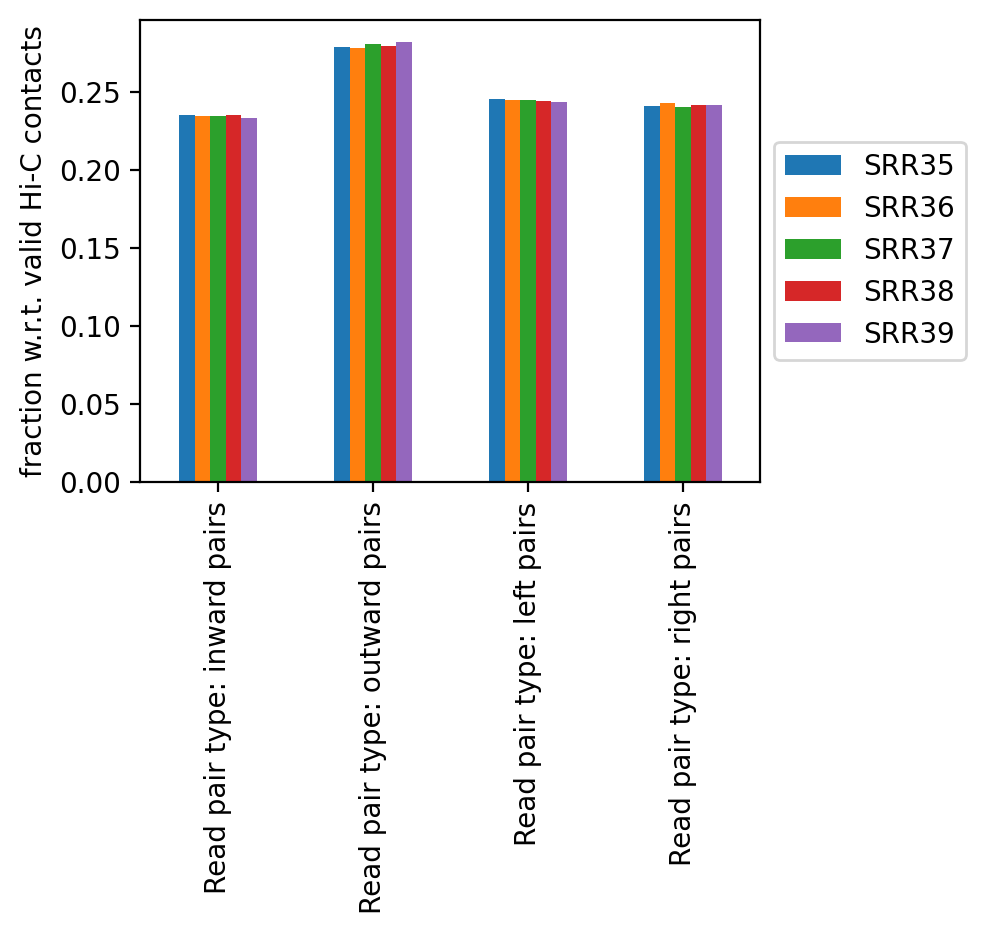
\includegraphics[keepaspectratio]{../steps/bwa/QC_all_samples/read_orientation.png}}

}

\subcaption{\label{fig-explorer-read-orientation}Read orientation}

\end{minipage}%
%
\begin{minipage}{0.33\linewidth}

\centering{

\pandocbounded{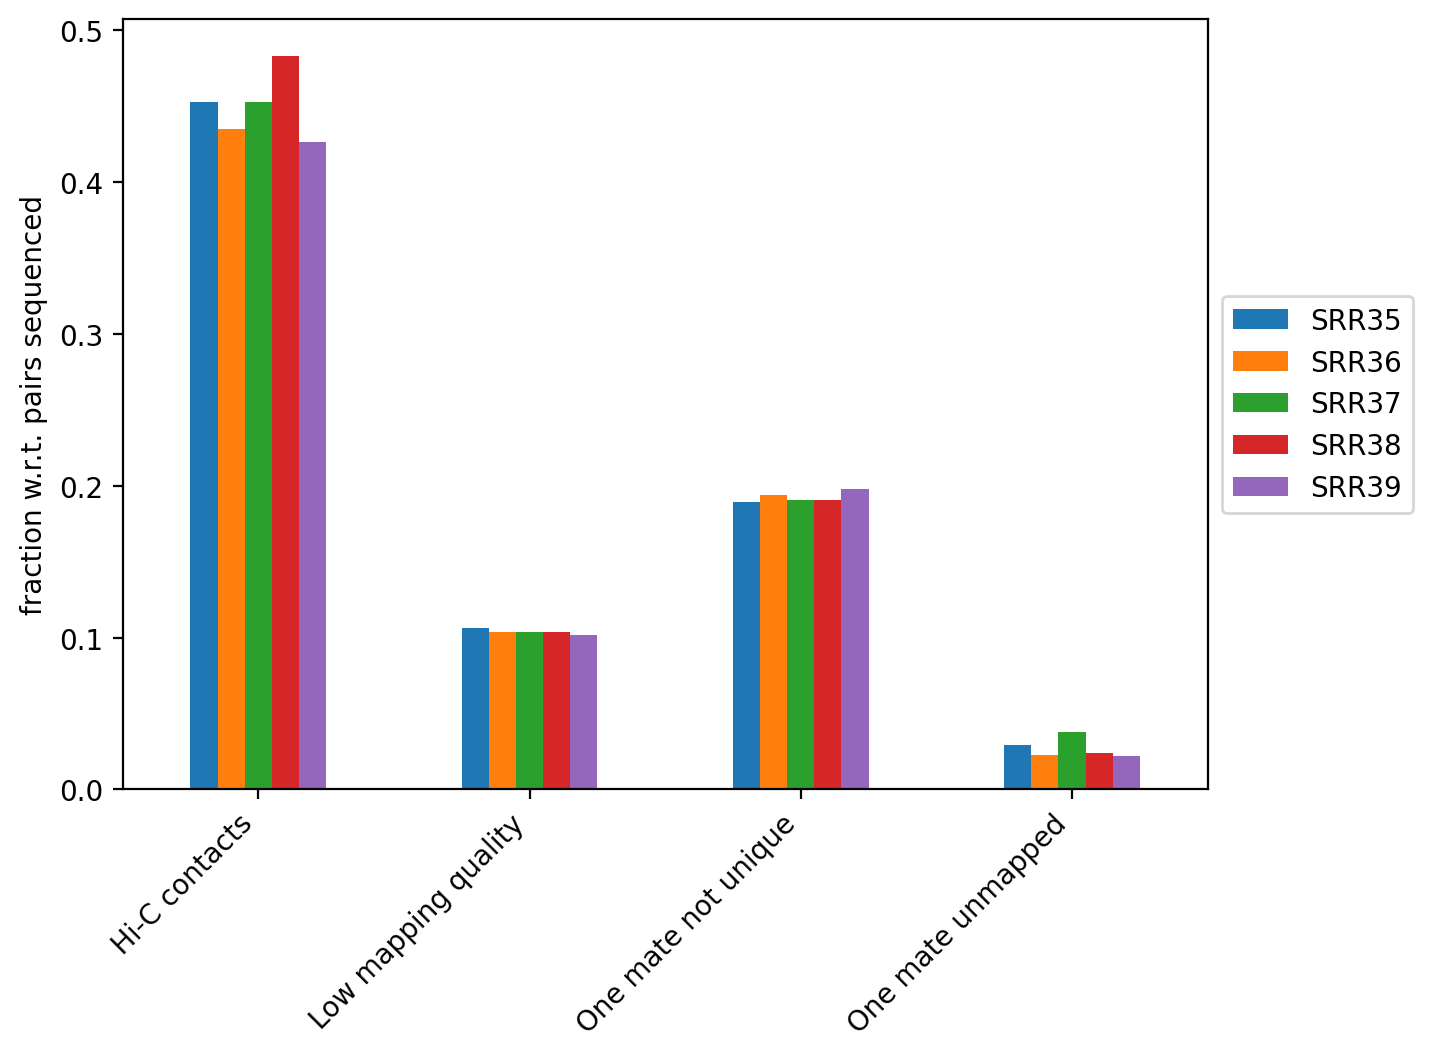
\includegraphics[keepaspectratio]{../steps/bwa/QC_all_samples/unmappable_and_non_unique.png}}

}

\subcaption{\label{fig-explorer-unique-pairs}Unique pairs}

\end{minipage}%
%
\begin{minipage}{0.33\linewidth}

\centering{

\pandocbounded{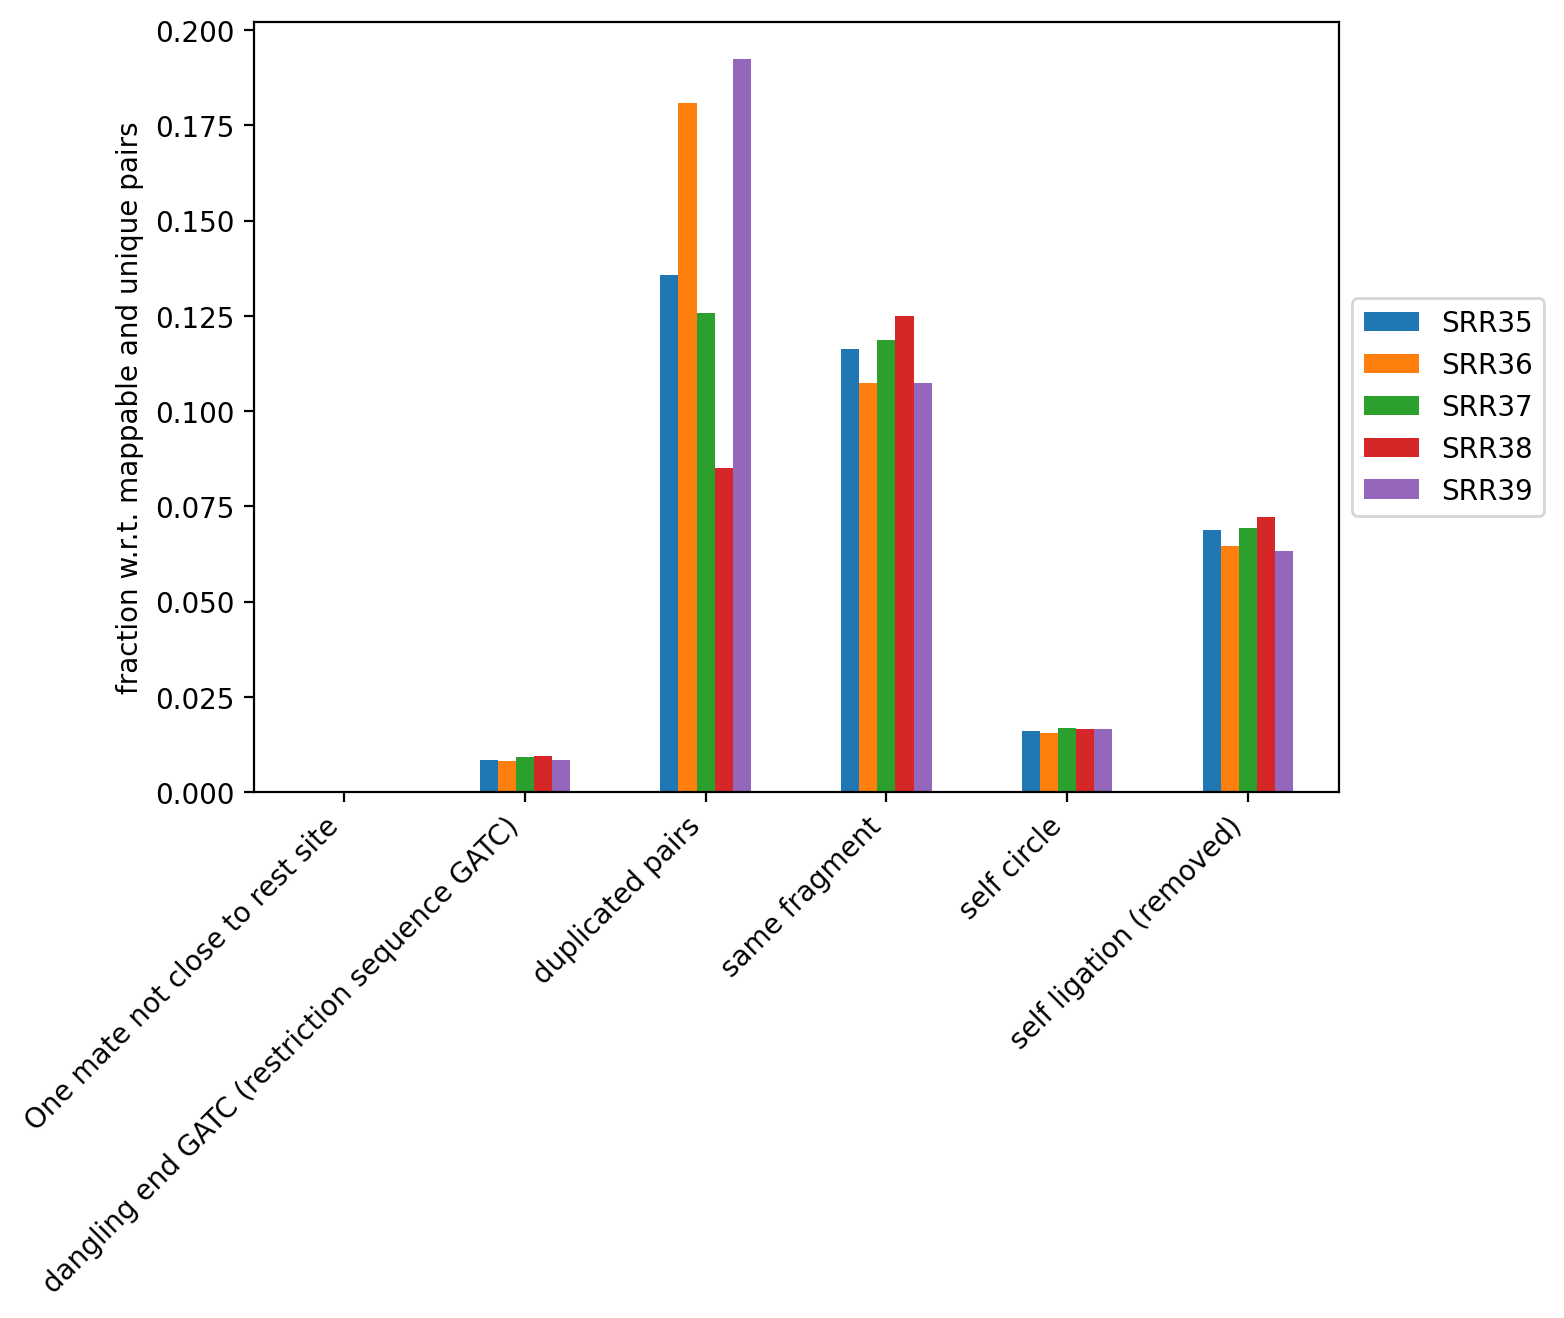
\includegraphics[keepaspectratio]{../steps/bwa/QC_all_samples/pairs_discarded.png}}

}

\subcaption{\label{fig-explorer-discarded-pairs}Discarded pairs}

\end{minipage}%
\newline
\begin{minipage}{0.33\linewidth}

\centering{

\pandocbounded{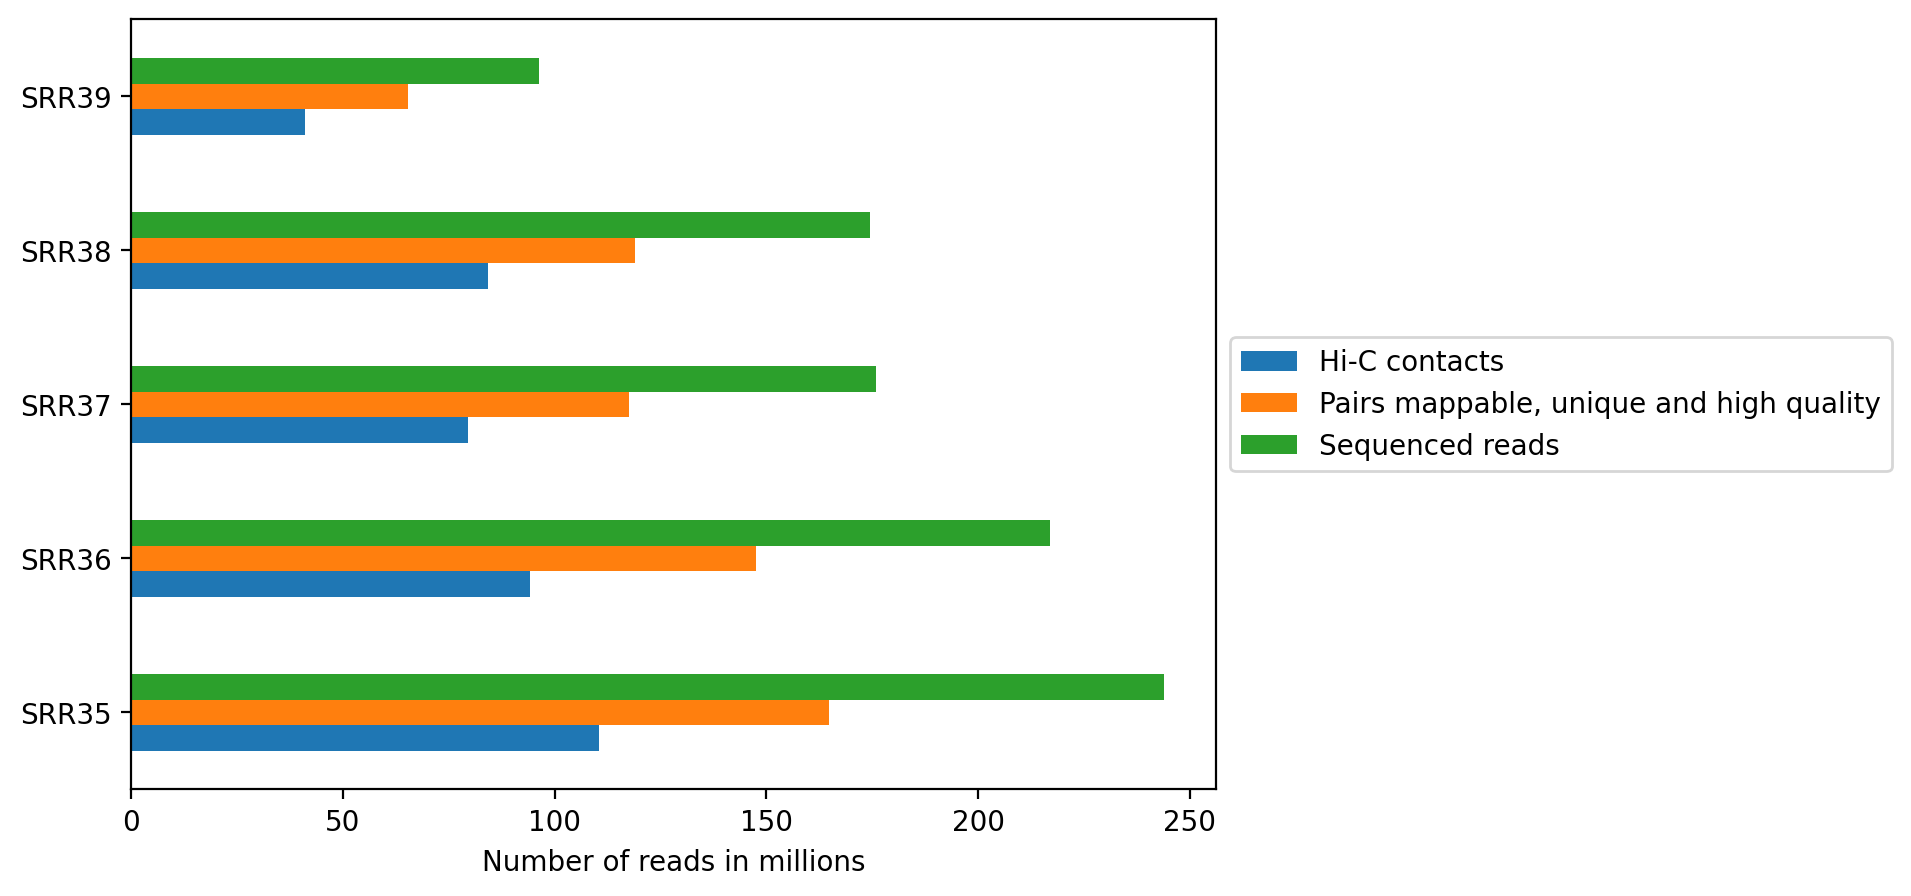
\includegraphics[keepaspectratio]{../steps/bwa/QC_all_samples/pairs_sequenced.png}}

}

\subcaption{\label{fig-explorer-pairs-sequenced}Pairs sequenced}

\end{minipage}%
%
\begin{minipage}{0.33\linewidth}

\centering{

\pandocbounded{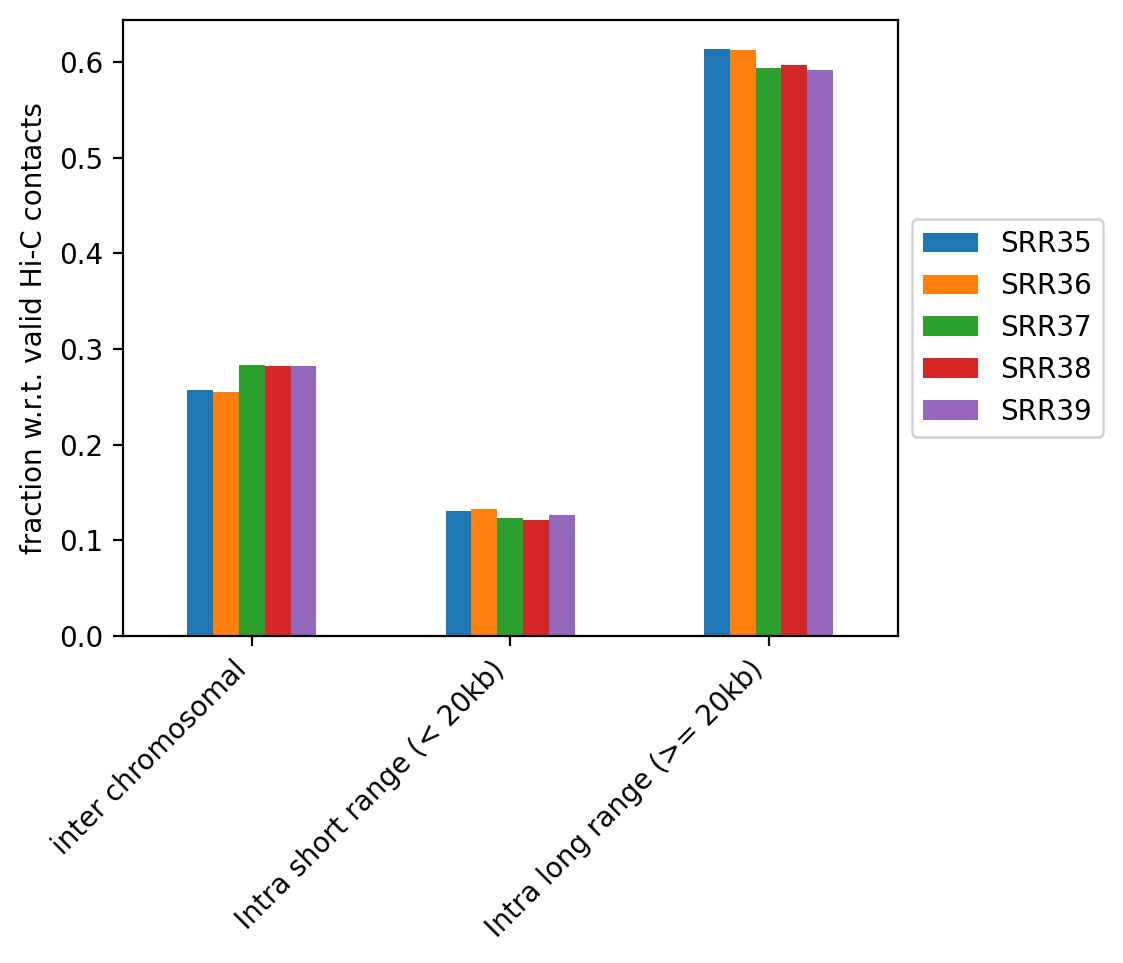
\includegraphics[keepaspectratio]{../steps/bwa/QC_all_samples/distance.png}}

}

\subcaption{\label{fig-explorer-contact-distance}Contact distance}

\end{minipage}%

\caption{\label{fig-explorer-qc}Quality control of the mapped Hi-C reads
using \emph{HiCExplorer} \texttt{hicQC}. The figures should be moved to
Supplementary/Appendix because they are ugly and un-alignable. But that
is the fault of HiCExplorer, not me. \st{Or I should spend a couple of
hours to plot them manually}.}

\end{figure}%

\subsection{Correction}\label{correction}

The correction diagnostic tool yielded a similar \emph{mad} threshold
within the range \([-3,-2]\). Even so, I followed the \emph{HicExplorer}
recommendation to set the lower threshold to at least -2 and the upper
threshold to 5 in the pre-normalization filter. I argue that with a high
number of valid contacts, it is safer to err on the side of caution and
maybe filter out bad data.

\begin{figure}

\begin{minipage}{0.06\linewidth}
~\end{minipage}%
%
\begin{minipage}{0.29\linewidth}

\centering{

\pandocbounded{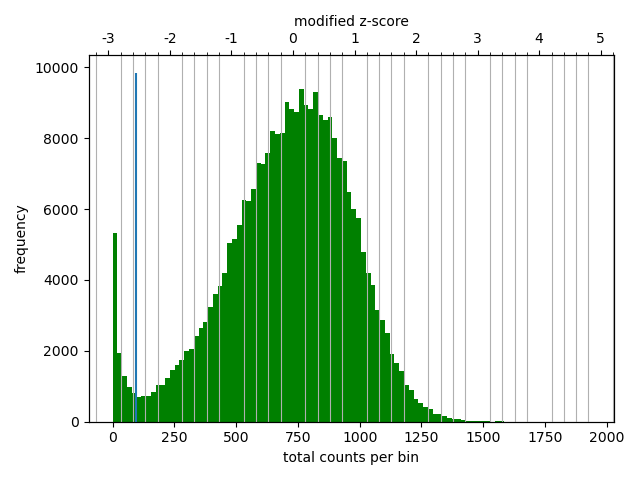
\includegraphics[keepaspectratio]{../figures/bwa/SRR6502335_diag_plot.png}}

}

\subcaption{\label{fig-explorer-pre-correction-SRR6502335}SRR6502335}

\end{minipage}%
%
\begin{minipage}{0.29\linewidth}

\centering{

\pandocbounded{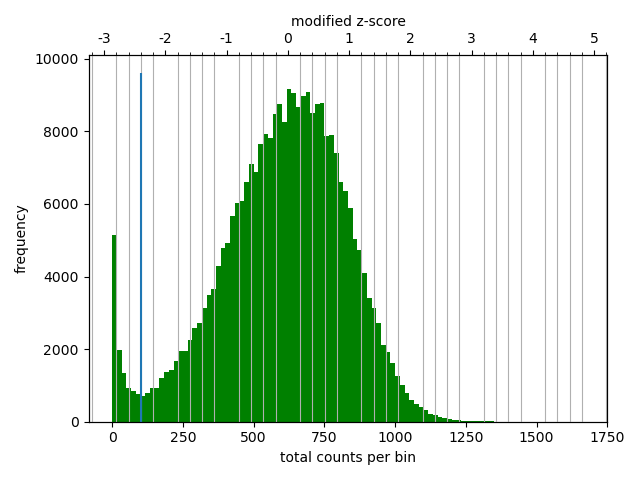
\includegraphics[keepaspectratio]{../figures/bwa/SRR6502336_diag_plot.png}}

}

\subcaption{\label{fig-explorer-pre-correction-SRR6502336}SRR6502336}

\end{minipage}%
%
\begin{minipage}{0.29\linewidth}

\centering{

\pandocbounded{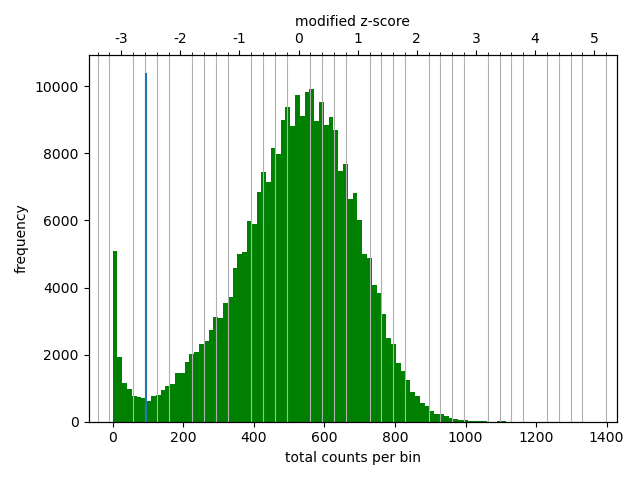
\includegraphics[keepaspectratio]{../figures/bwa/SRR6502337_diag_plot.png}}

}

\subcaption{\label{fig-explorer-pre-correction-SRR6502337}SRR6502337}

\end{minipage}%
%
\begin{minipage}{0.06\linewidth}
~\end{minipage}%
\newline
\begin{minipage}{0.21\linewidth}
~\end{minipage}%
%
\begin{minipage}{0.29\linewidth}

\centering{

\pandocbounded{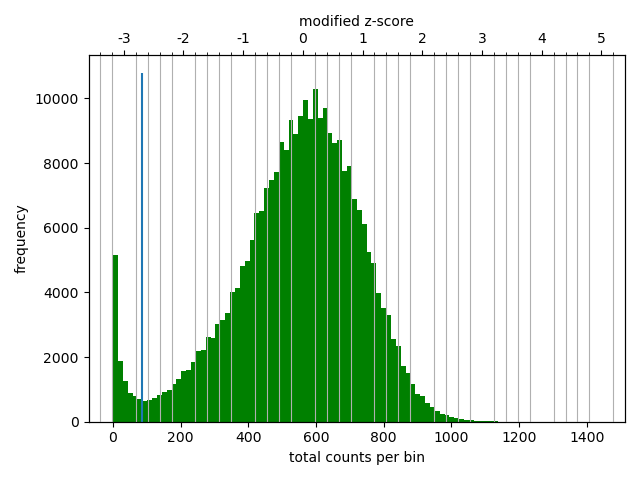
\includegraphics[keepaspectratio]{../figures/bwa/SRR6502338_diag_plot.png}}

}

\subcaption{\label{fig-explorer-pre-correction-SRR6502338}SRR6502338}

\end{minipage}%
%
\begin{minipage}{0.29\linewidth}

\centering{

\pandocbounded{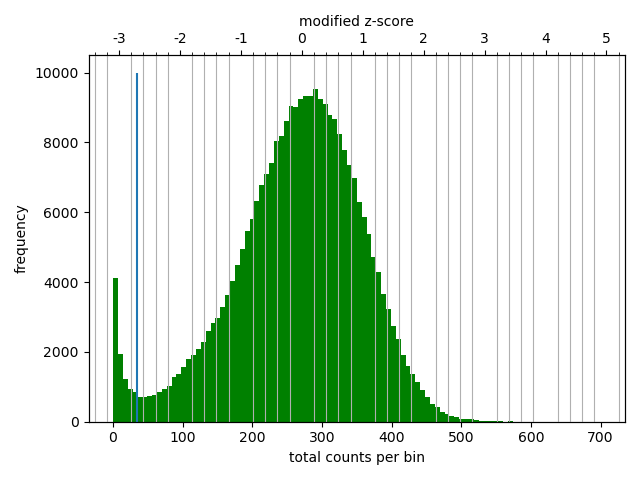
\includegraphics[keepaspectratio]{../figures/bwa/SRR6502339_diag_plot.png}}

}

\subcaption{\label{fig-explorer-pre-correction-SRR6502339}SRR6502339}

\end{minipage}%
%
\begin{minipage}{0.21\linewidth}
~\end{minipage}%

\caption{\label{fig-explorer-pre-correction}Histograms of the number of
counts per bin (bottom x-axis) and the modified z-score (top x-axis)
from which the \emph{mad} threshold is defined.}

\end{figure}%

\begin{quote}
NB: when I say that a mapper performs poorly in finding Hi-C contacts,
it is \texttt{hicBuildMatrix} that performs badly when reads are mapped
with that mapper.
\end{quote}

To compare these mappings with others, the QC results is an easy way.
Therefore, the reads were mapped with \emph{bowtie2} in both end-to-end-
and local-mode followed by \texttt{hiCBuildMatrix}, and the QC from each
method was plotted next to each other
(Figure~\ref{fig-explorer-all-3-qc}). Interestingly, \emph{bowtie2} was
much more computer-intensive in both modes, perhaps because of the
\texttt{-\/-very-sensitive} option. In any case, the QC reveals a major
difference in the total number of reads that are determined to be valid
Hi-C contacts by \texttt{hicBuildMatrix}. As expected,
\emph{end-to-end-bowtie2} performs worse at locating Hi-C contacts than
the other methods {[}ref row1{]}, finding a very low amount of mappable,
unique pairs passing the quality threshold. In contrast,
\emph{local-bowtie2} performs similarly to \emph{bwa} in finding
mappable, unique, high-quality pairs, but calls only approximately half
the number of valid Hi-C contacts (\textgreater20\%), resulting in a
fraction of valid Hi-C pairs that hits the expectation from
\emph{HicExplorer} docs {[}ref row3{]}. With \emph{bwa}, the reads were
discarded either due to low mapping quality or non-unique mates, whereas
with \emph{local-bowtie2}, the reads were almost exclusively filtered
out due to low mapping quality. This must be a result of how the mappers
assign mapping quality, and I believe \emph{local-bowtie2} looks
suspiciously selective in finding unique but low quality alignments.
\emph{end-to-end-bowtie} almost exclusively filters out read-pairs where
one mate is unmapped, which is expected when the majority of reads are
unmapped.

\begin{figure}[H]

\centering{

\pandocbounded{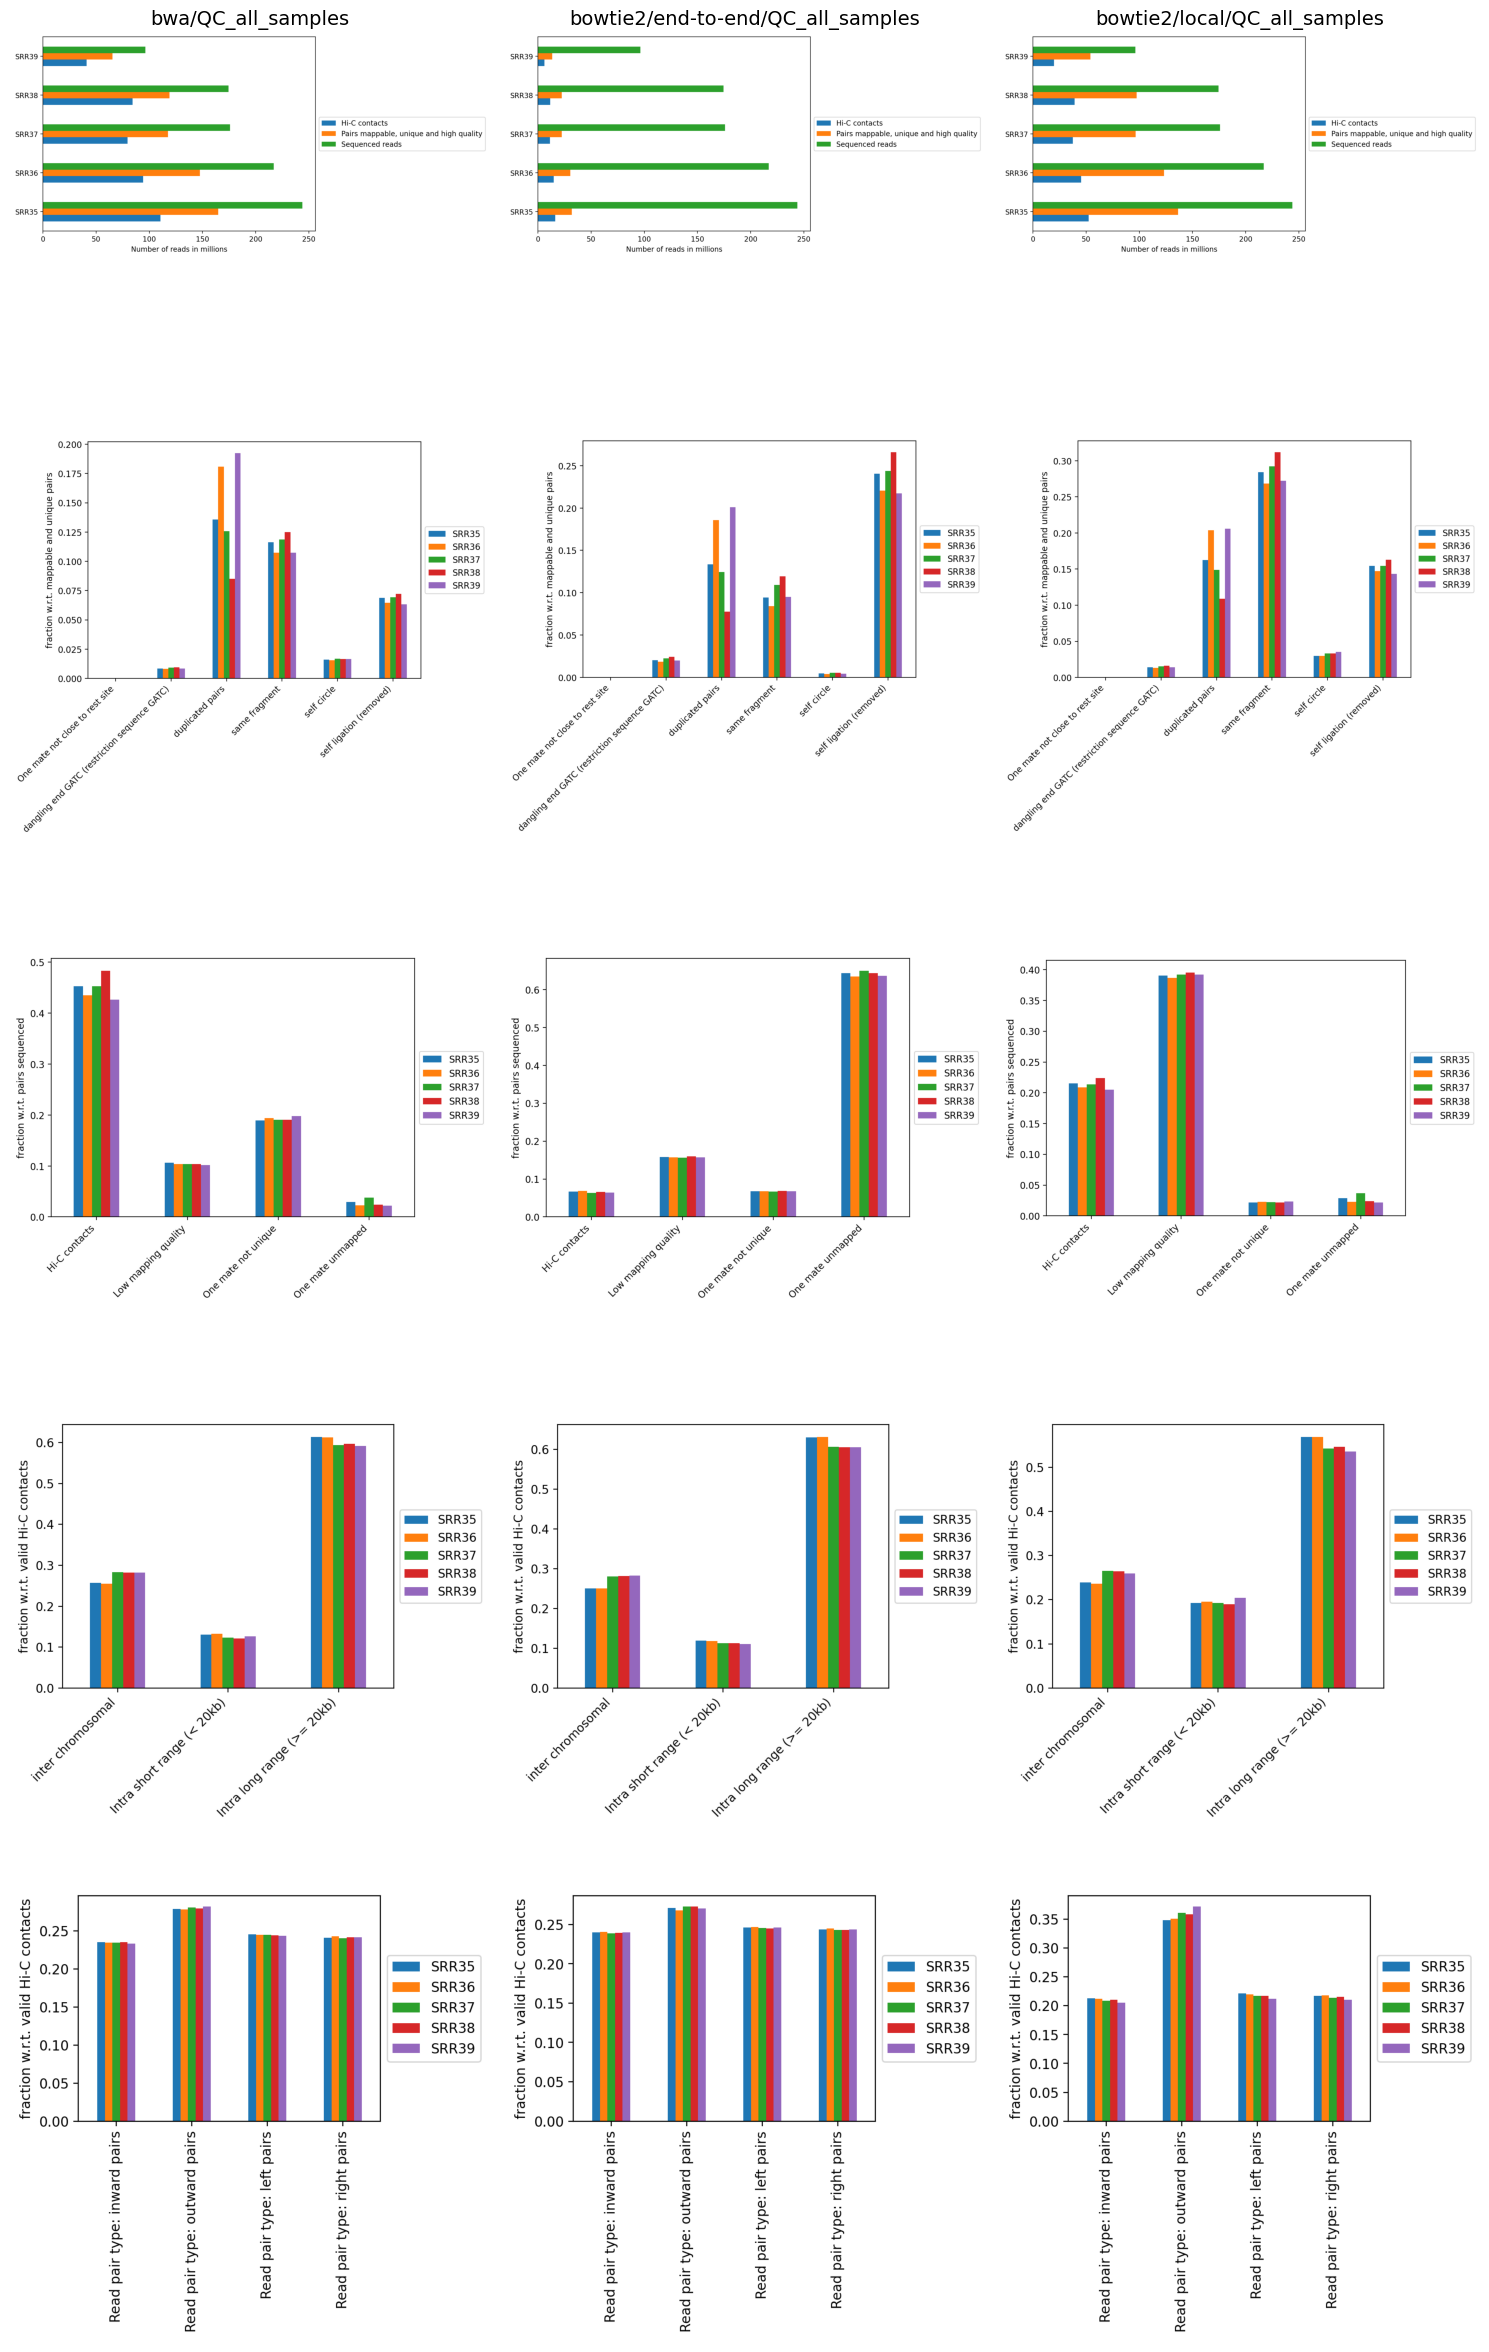
\includegraphics[keepaspectratio]{index_files/figure-latex/..-notebooks-01_hicexplorer-fig-explorer-all-3-qc-output-1.png}}

}

\caption{\label{fig-explorer-all-3-qc}Comparison of HiCExplorer QC plots
for all samples using different alignment tools.}

\end{figure}%

As discussed, the five samples were pooled with \texttt{hicSumMatrices},
and the non-standard contigs (unplaced scaffolds) were filtered out, and
the different resolutions were created (\texttt{hicMergeMatrixBins}).
\emph{HiCExplorer} also comes with a normalization function prior to
correcting the matrix, which should be applied if different samples
should have comparable bin counts. It has no effect when having only one
matrix. Nevertheless, the pooled matrix was normalized and then
corrected compared in Figure~\ref{fig-explorer-pooled-norm-normcorr}.

\begin{figure}

\begin{minipage}{0.50\linewidth}

\centering{

\pandocbounded{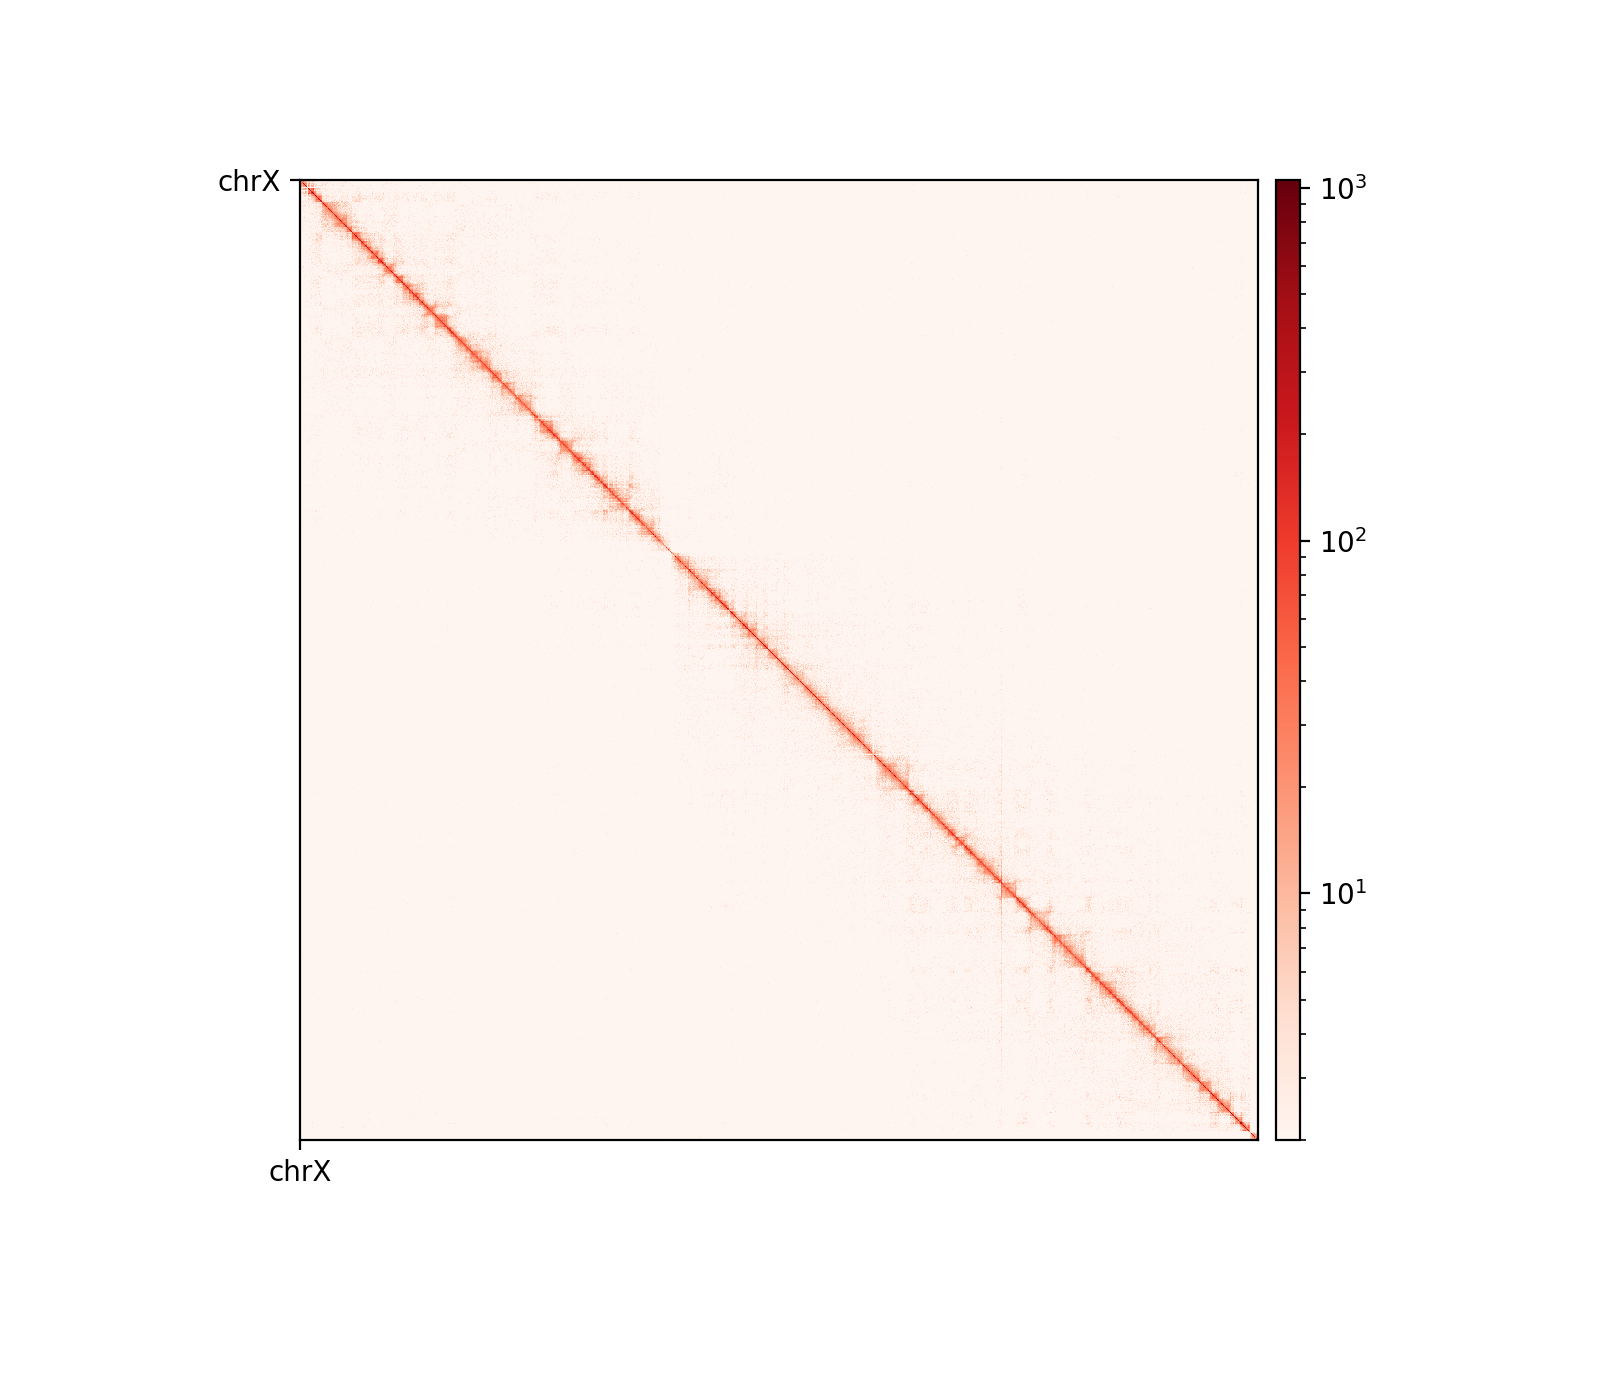
\includegraphics[keepaspectratio]{../figures/bowtie2/local/filter_pooled_50kb_chrX.png}}

}

\subcaption{\label{fig-explorer-pooled-chrX-norm}Normalized matrix chrX}

\end{minipage}%
%
\begin{minipage}{0.50\linewidth}

\centering{

\pandocbounded{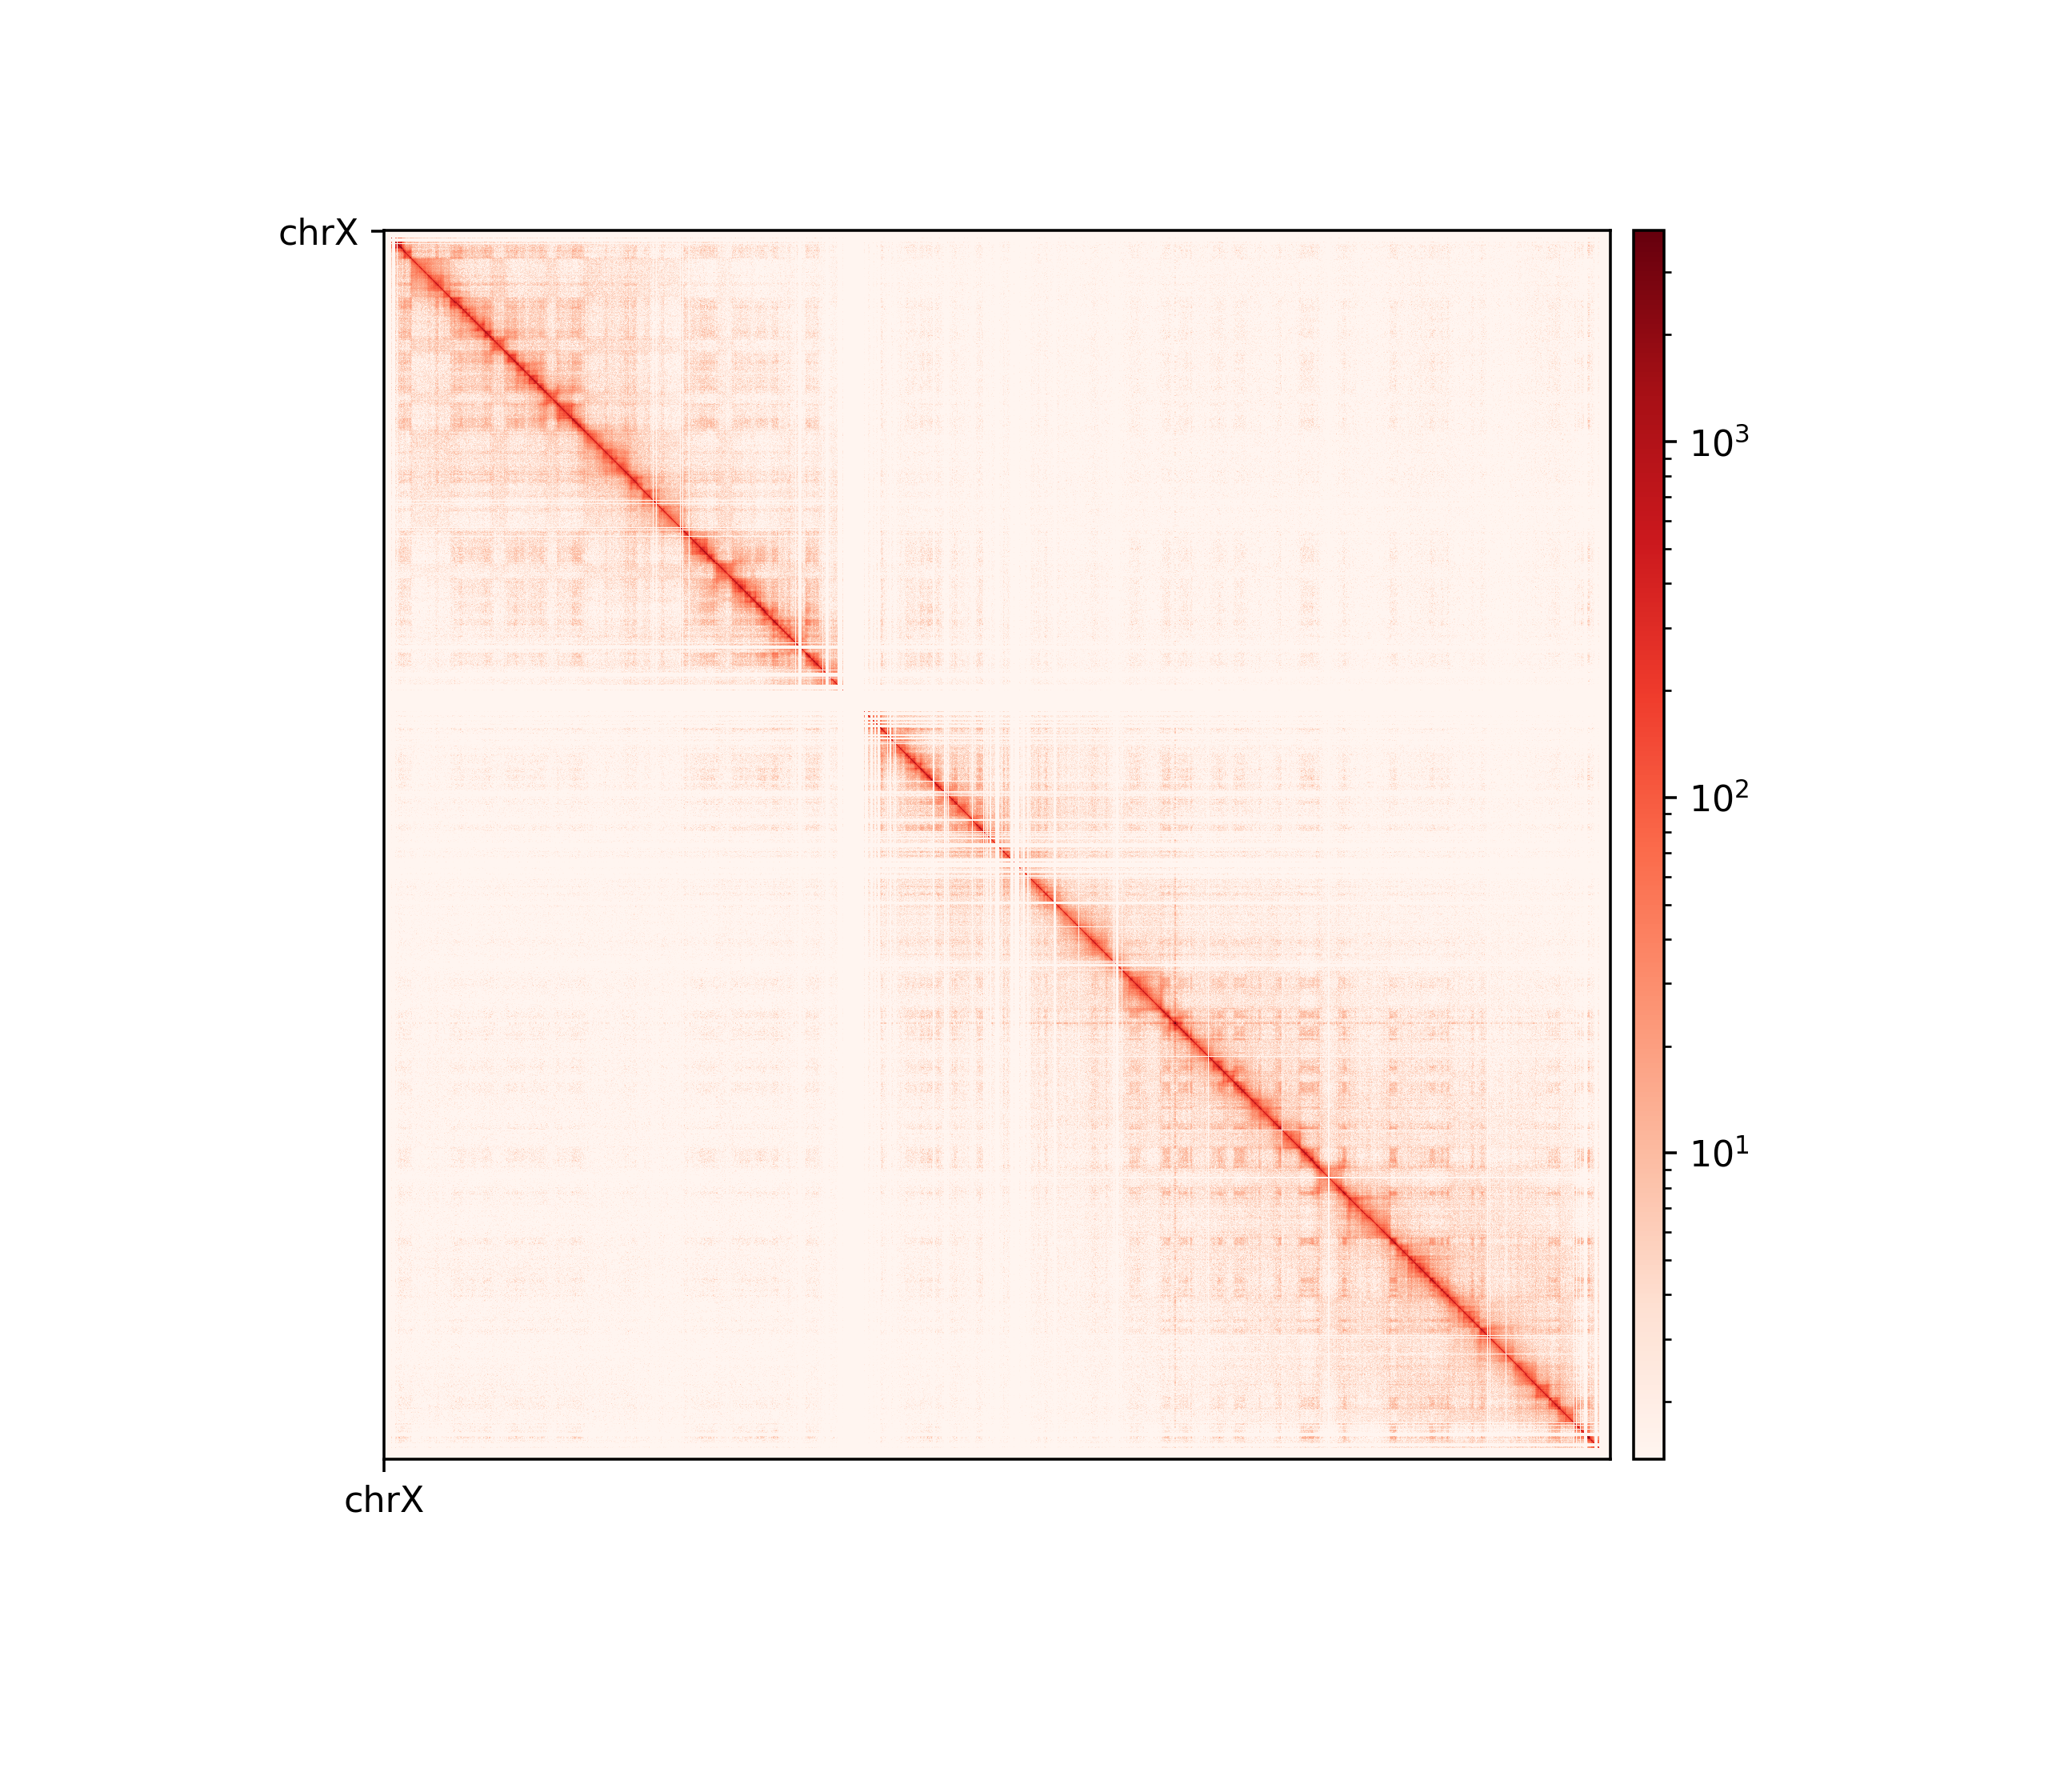
\includegraphics[keepaspectratio]{../figures/bowtie2/local/normalized/normsm_filter_pooled_100kb_corrected_chrX-full.png}}

}

\subcaption{\label{fig-explorer-pooled-chrX-normcorr}Normalized and
corrected chrX}

\end{minipage}%

\caption{\label{fig-explorer-pooled-norm-normcorr}A comparison of
interaction matrices before/after iterative correction
(\emph{HiCExplorer}).}

\end{figure}%

It is now obvious why we have to correct the matrix. The uncorrected
(Figure~\ref{fig-explorer-pooled-chrX-norm}) has no signal apart from
the diagonal. Even though some bins have been filtered out, the expected
\emph{plaid} pattern of a contact matrix is visible along the diagonal
after the correction (Figure~\ref{fig-explorer-pooled-chrX-normcorr}),
leaving evidence for chromatin structure, especially in the first 50
million bases of the chromosome. There is a wide region of empty values
at the place of the centromere.

\subsection{Eigenvectors}\label{eigenvectors}

The PCA performed by \texttt{hicPCA} on the pooled samples at both 50kb
and 100kb resolution yielded the first 3 principal components. For PC1
on both resolutions (Figure~\ref{fig-explorer-pc1-50kb},
Figure~\ref{fig-explorer-pc1-100kb}) we observe only a single sign
change which occurs at around 60 Mbp, the region of the centromere. It
means the PCA has captured more variance between the chromosome arms
than within them, making it uninformative about chromatin compartments.
Upon visual inspection, it is clear that neither of the PC graphs
capture the pattern of the interaction matrix by its change of sign. It
seems the PCs capture variance from a bias that varies slowly and
predictably along the chromosome. The first PC that is supposed to
capture the compartments very suspiciously changes sign at the region of
the centromere, a classic problem that could be solved by restricting
the values from which the PC is calculated along the chromosome.
Unimpressed, I rationalize that the option \texttt{-\/-extra-track} to
provide a gene track or histone coverage should not affect this result
much. It should be provided as a phasing track to orient the eigenvector
to positively correlate with gene density or histone marks, and could
possibly muddle the compartments if not included. At this point, I
stoppped using \emph{HiCExplorer}, as I assessed that a more flexible
tool was needed.

\begin{figure}

\begin{minipage}{0.33\linewidth}

\centering{

\pandocbounded{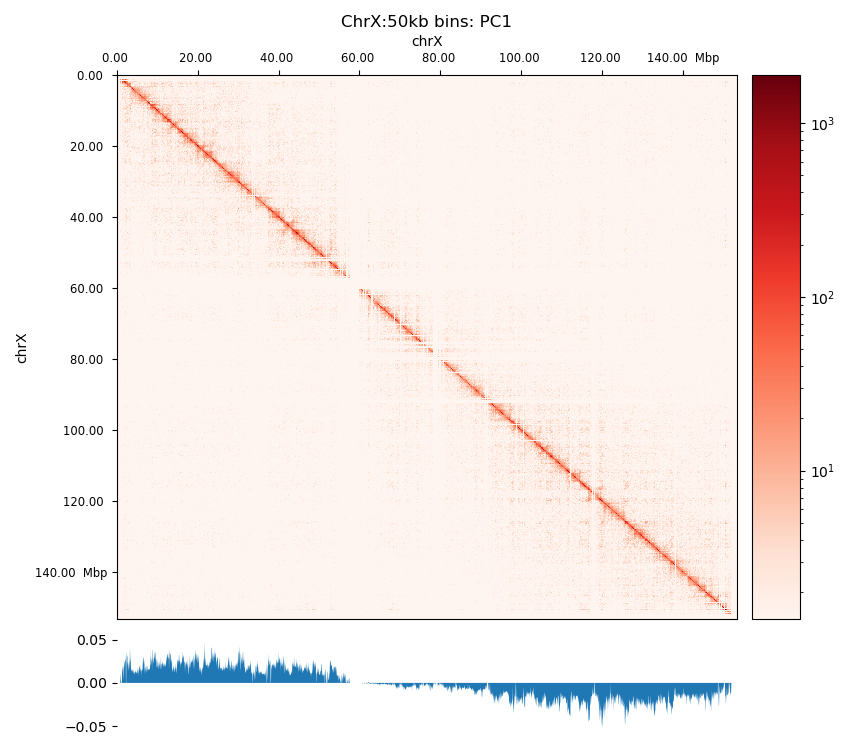
\includegraphics[keepaspectratio]{../figures/bowtie2/local/normalized/pc1_50kb_corrected_chrX.png}}

}

\subcaption{\label{fig-explorer-pc1-50kb}}

\end{minipage}%
%
\begin{minipage}{0.33\linewidth}

\centering{

\pandocbounded{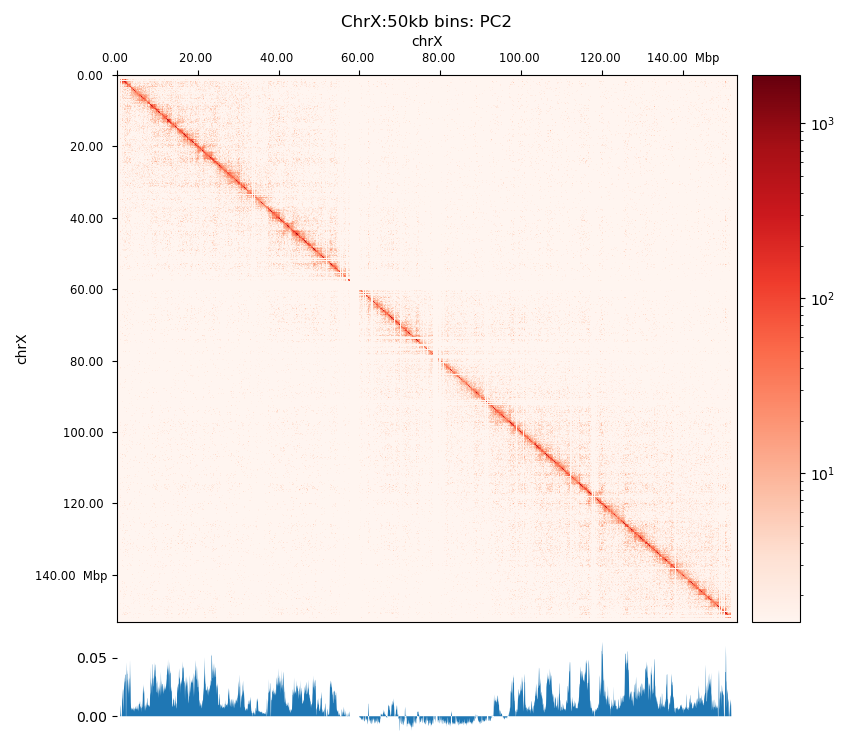
\includegraphics[keepaspectratio]{../figures/bowtie2/local/normalized/pc2_50kb_corrected_chrX.png}}

}

\subcaption{\label{fig-explorer-pc2-50kb}}

\end{minipage}%
%
\begin{minipage}{0.33\linewidth}

\centering{

\pandocbounded{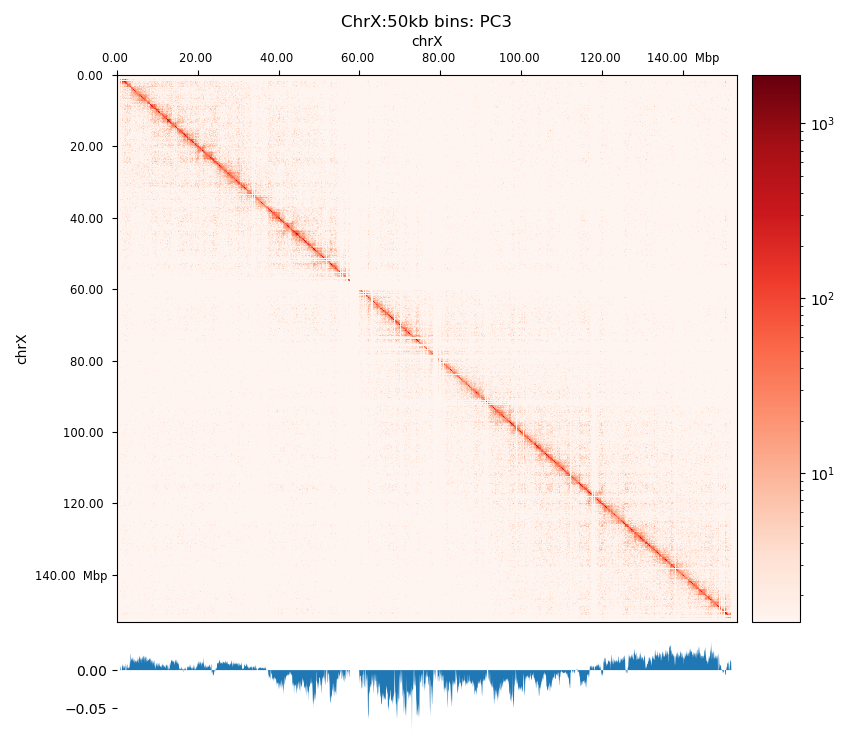
\includegraphics[keepaspectratio]{../figures/bowtie2/local/normalized/pc3_50kb_corrected_chrX.png}}

}

\subcaption{\label{fig-explorer-pc2-50kb}}

\end{minipage}%
\newline
\begin{minipage}{0.33\linewidth}

\centering{

\pandocbounded{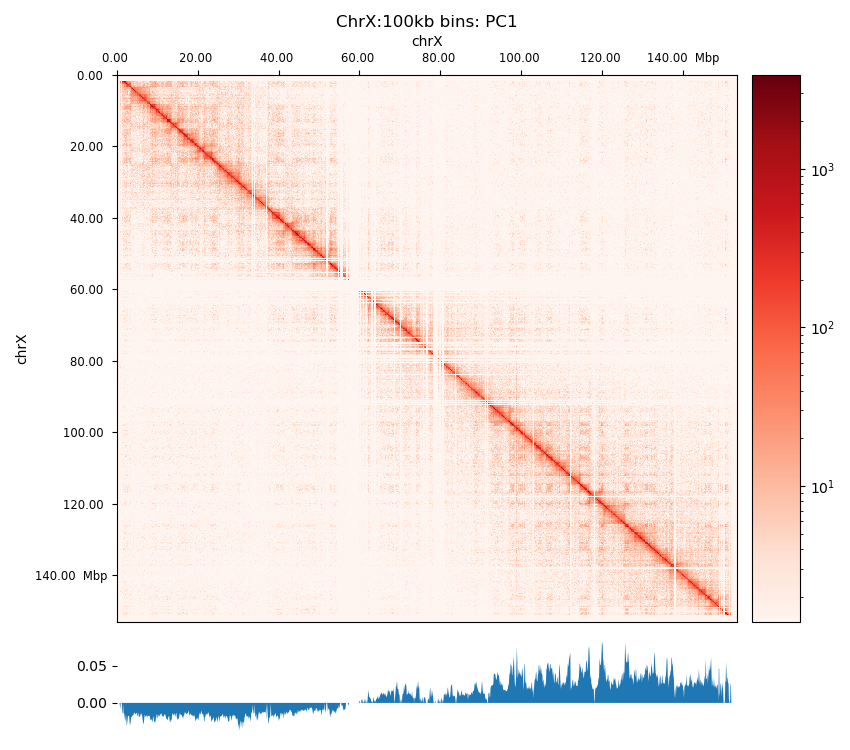
\includegraphics[keepaspectratio]{../figures/bowtie2/local/normalized/pc1_100kb_corrected_chrX.png}}

}

\subcaption{\label{fig-explorer-pc1-100kb}}

\end{minipage}%
%
\begin{minipage}{0.33\linewidth}

\centering{

\pandocbounded{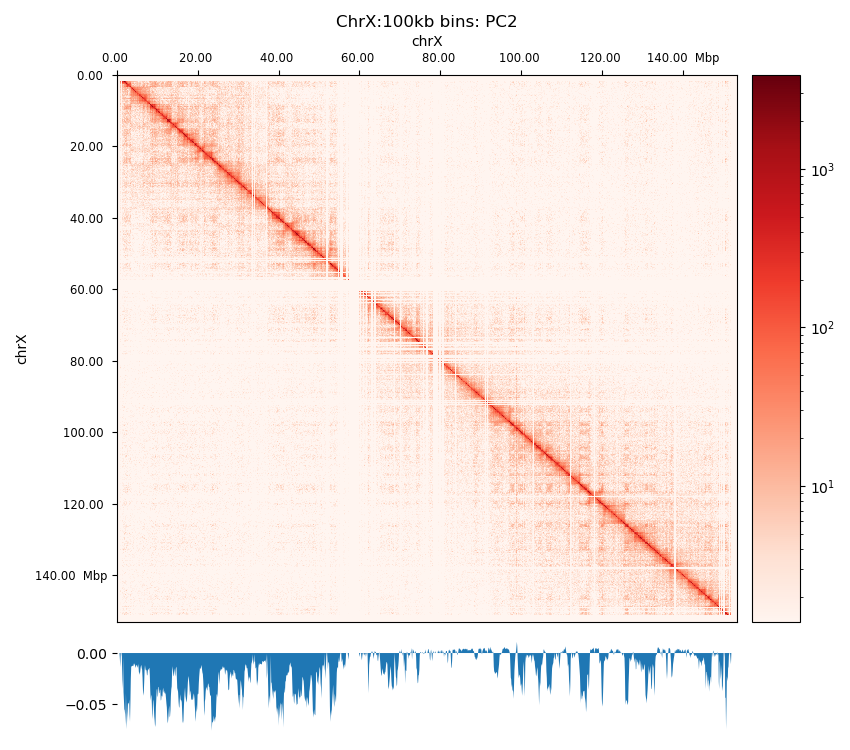
\includegraphics[keepaspectratio]{../figures/bowtie2/local/normalized/pc2_100kb_corrected_chrX.png}}

}

\subcaption{\label{fig-explorer-pc2-100kb}}

\end{minipage}%
%
\begin{minipage}{0.33\linewidth}

\centering{

\pandocbounded{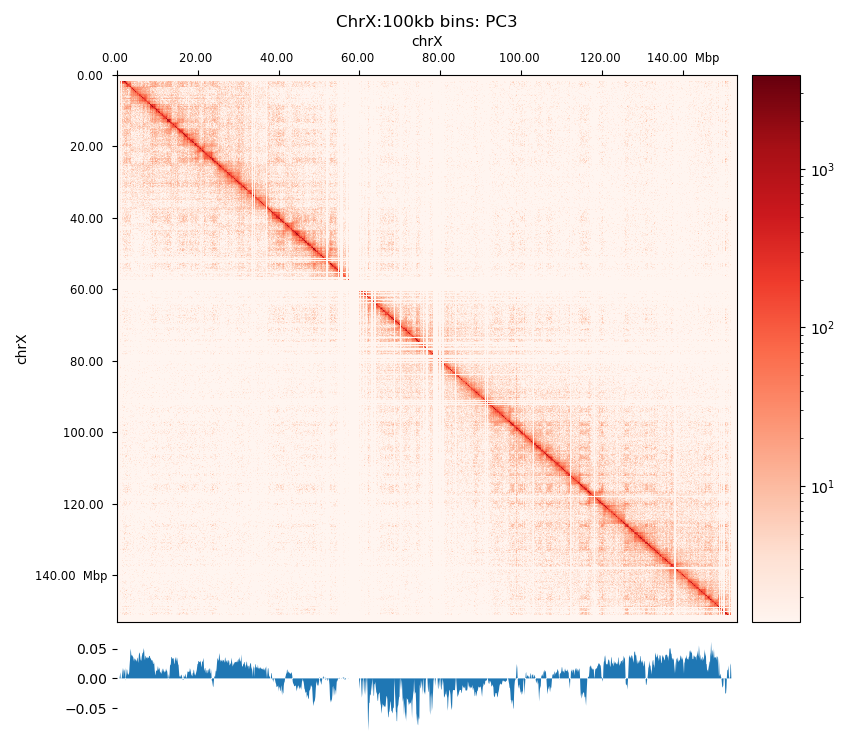
\includegraphics[keepaspectratio]{../figures/bowtie2/local/normalized/pc3_100kb_corrected_chrX.png}}

}

\subcaption{\label{fig-explorer-pc3-100kb}}

\end{minipage}%

\caption{\label{fig-explorer-pca}Corrected interaction matrix for
chromosome X along with PC1, 2, or 3, respectively. a-c: 50kb
resolution, d-f: 100kb resolution. \emph{HiCExplorer}.}

\end{figure}%

\section{Open2c ecosystem}\label{open2c-ecosystem}

\subsection{Quality Control}\label{quality-control-1}

\subsubsection{\texorpdfstring{Initial run
(\texttt{-\/-walks-policy\ mask})}{Initial run (-\/-walks-policy mask)}}\label{initial-run---walks-policy-mask}

Comparing the multiQC report for each of the cell sources show similar
distributions of \emph{unmapped} (both sides unmapped), \emph{one-sided}
(one side mapped), \emph{two-sided} (both sides mapped), and
\emph{duplicated} (w.r.t. total mapped) reads. The percentage of
\emph{cis} pairs w.r.t. mapped pairs is around 70\% for all samples.
{[}ref supptbl-qc-all-samples-mask{]}. The valid pairs also show similar
distributions of pair types divided into 10 categories. The \(P(s)\)
curve looks similar as well, peaking between 270 bp and 320 bp
separation (ref suppfig-multiqc-ps-curve). The QC does not show any
information about mapping quality of the reads. Note that the \(P(s)\)
ccurve arise from pre-filtered pairs, and should be compcared with the
\(P(s)\) of the cooler after filtering.

{[}ref if there is time, include a histogram of mapq values for pairs{]}

\subsubsection{\texorpdfstring{Recommended
(\texttt{-\/-walks-policy\ 5unique})}{Recommended (-\/-walks-policy 5unique)}}\label{recommended---walks-policy-5unique}

Parsing alignments with the recommended walks-policy aproximately halves
the percentage of \emph{unmapped} reads, and \emph{one-} and
\emph{two-sided} reads as well \emph{duplicated} reads are slightly
increased. Overall number of unique pairs are increased with more than
20\% increase. The percentage of \emph{cis} pairs are only decreased by
a percentage point at most {[}ref supptbl-qc-all-samples-5unique{]}.

\subsection{Correction}\label{correction-1}

Matrix balancing did not show major improvement in the plaid pattern, as
it was already pretty good. It does, however, filter out bins that are
deemed too low-count to be informative, for example peri-centromeric
regions. The matrix was expected to be smoother after balancing (for
chromosomes), as regions along a chromosome should only vary slowly in
contact frequency with other regions {[}ref{]}.

\begin{figure}[H]

\centering{

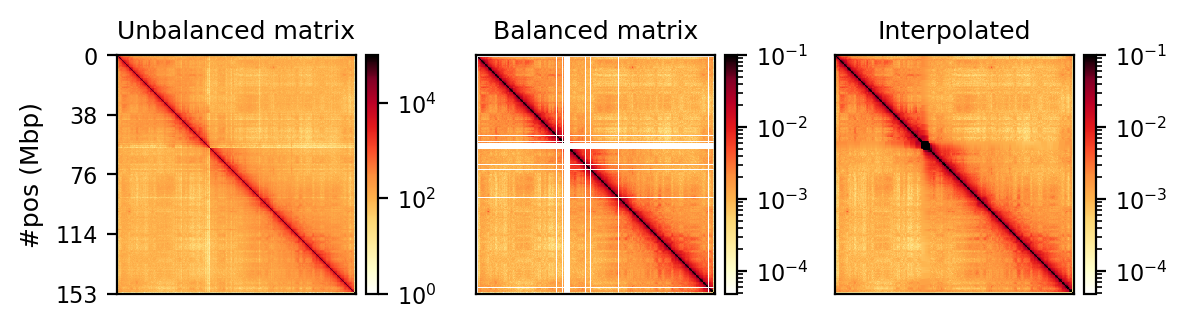
\includegraphics[width=6.17708in,height=1.70833in]{index_files/figure-latex/..-notebooks-05_rec_compartments-fig-rs-chrx-raw-balanced-cgi-output-2.png}

}

\caption{\label{fig-rs-chrx-raw-balanced-cgi}Raw, balanced, and
interpolated chrX interaction matrix in 500kb resolution. The
interpolation is done to make the matrix more visually appealing, but it
is not necessary for the analysis.}

\end{figure}%

\begin{figure}[H]

\centering{

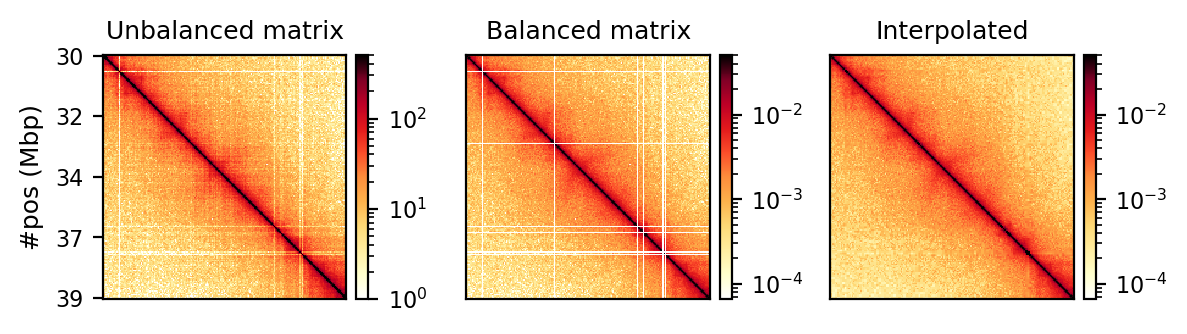
\includegraphics[width=6.17708in,height=1.73958in]{index_files/figure-latex/..-notebooks-05_rec_compartments-fig-rs-chrx-raw-balanced-cgi-subset-output-2.png}

}

\caption{\label{fig-rs-chrx-raw-balanced-cgi-subset}Raw, balanced, and
interpolated chrX interaction matrix in 50kb resolution. The
interpolation is done to make the matrix more visually appealing, but it
is not necessary for the analysis.}

\end{figure}%

The coarsegrained and interpolated matrix is useful to make a
good-looking interaction matrix, but is not that useful for analysis
purposes. It might get easier to visually inspect the matrix, but it is
not clear how well the interpolated matrix reflects the structure of the
chromatin. The regions that are coarsgrained are small zero- or
low-count bins which are averaged, effectively reducing the resolution
of those regions until the count is sufficient. They get more frequent
the longer genomic distance (the further we travel from the diagonal),
and effectively enables us to get some intuition about the interactions.
The coarsegrain, however, does not interpolate the \texttt{NaN}s created
when filtering out whole bins in the balancing step (horisontal and
vertical lines in Figure~\ref{fig-rs-chrx-raw-balanced-cgi} and
Figure~\ref{fig-rs-chrx-raw-balanced-cgi-subset}; middle). This is done
in a subsequent step by linearly interpolating the \texttt{NaN}s.
Examining the interpolated matrix on full chrX
(Figure~\ref{fig-rs-chrx-raw-balanced-cgi}; right) gives the impression
that the pericentromeric (at \textasciitilde60 Mbp) region harbours a
\emph{very} strong compartment, but that is clearly an artefact of the
interpolation on the very large empty region of the centromere, where
the diagonal is somehow extended in a square. On the thinner lines, the
interpolation seem to be more smooth, and barely noticable on the
diagonal.

\subsubsection{\texorpdfstring{\texttt{NaN}
histograms}{NaN histograms}}\label{nan-histograms}

As expected, most of the low quality bins are located on the edges of
the chromosome arms, especially the region around the centromere {[}ref
litterature{]}, as they contain many repetitive sequences. The
low-quality bins are filtered out by the balancing algorithm, those bins
are \texttt{NaN} in the Hi-C matrix. The median position of the
\texttt{NaN} values (Figure~\ref{fig-e1_nan_hist}) ranges between \(58\)
and \(63.5\), which is within the estimate of the centromeric region of
\emph{rhemac10}.

\begin{figure}[H]

\centering{

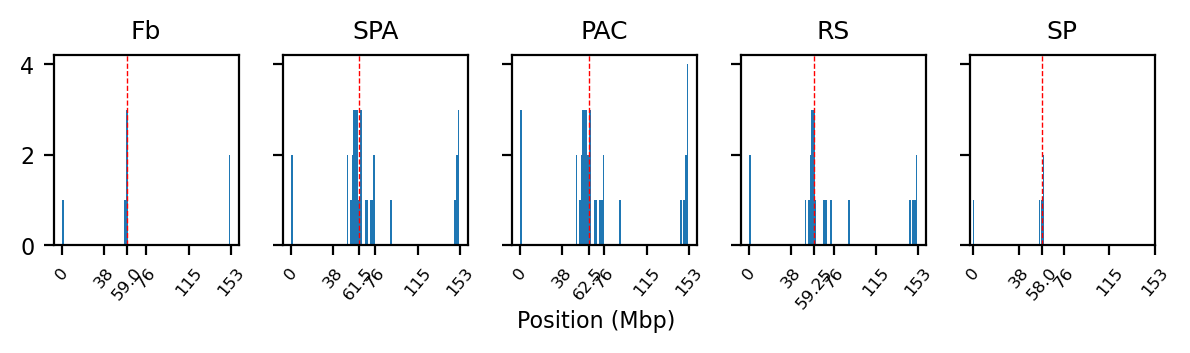
\includegraphics[width=6.19792in,height=1.83333in]{index_files/figure-latex/..-notebooks-05_rec_compartments-fig-e1_nan_hist-output-1.png}

}

\caption{\label{fig-e1_nan_hist}Histogram of NaN values in the E1
eigenvector for each cell type. Median position is marked with a red
dashed line.}

\end{figure}%

The fact that the medians lie within the centromeric region on all cell
sources shows both that the majority of the bad bins are in the
(peri)centromeric region \emph{and} there are approximately equally many
on each side.

\subsection{Compartments
(Eigenvectors)}\label{compartments-eigenvectors}

The three viewframes (\emph{Full}, \emph{Arms}, \emph{10Mb}) for the
calculation of the eigenvectors captured different variability in the
data (Figure~\ref{fig-e1-matrix-500kb-full-arms-10mb-round_spermatid}),
and as expected, the inferred compartments (colored red on the E1
tracks) are more abundant and smaller with smaller viewframes. To
determine how well each of the E1 tracks capture the pattern in the
interaction matrix, we can overlay the matrix with the E1 sign-change
and visually determine if the squares reflect the E1 sign change
(Figure~\ref{fig-e1-matrix-500kb-full-arms-10mb-round_spermatid}).

\begin{figure}[H]

\begin{minipage}{0.48\linewidth}

\centering{

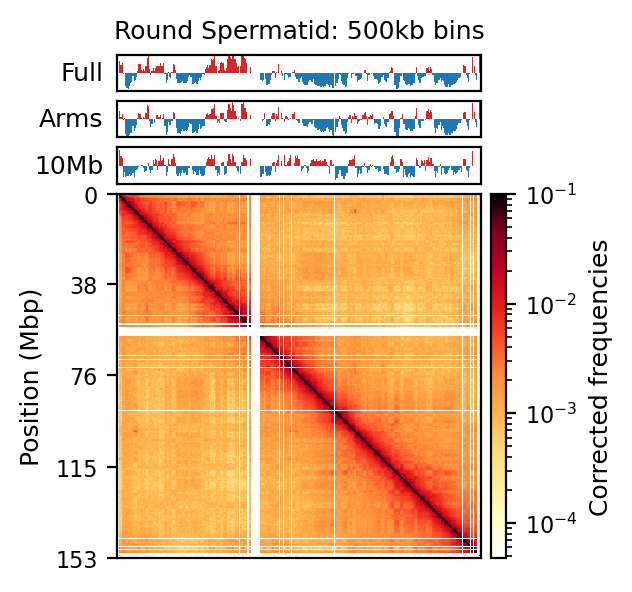
\includegraphics[width=3.29167in,height=3.08333in]{index_files/figure-latex/..-notebooks-05_rec_compartments-fig-e1-matrix-500kb-full-arms-10mb-round_spermatid-output-1.png}

}

\subcaption{\label{fig-e1-matrix-500kb-full-arms-10mb-round_spermatid}E1
eigenvector values for merged round spermatid samples at 500kb
resolution, as well as the interaction matrix. E1 was restricted to
either Full-chromosome (top), Chromosome-arms (middle), or 10Mb windows
(bottom).}

\end{minipage}%
%
\begin{minipage}{0.03\linewidth}
~\end{minipage}%
%
\begin{minipage}{0.48\linewidth}

\centering{

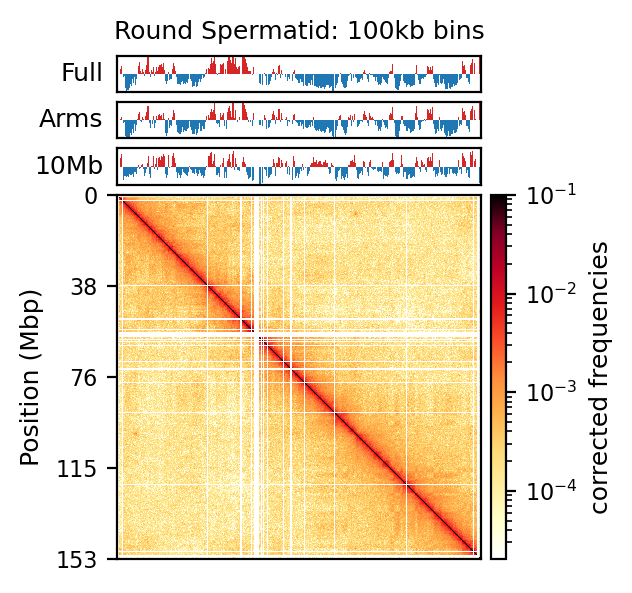
\includegraphics[width=3.29167in,height=3.08333in]{index_files/figure-latex/..-notebooks-05_rec_compartments-fig-e1-matrix-100kb-full-arms-10mb-round_spermatid-output-1.png}

}

\subcaption{\label{fig-e1-matrix-100kb-full-arms-10mb-round_spermatid}E1
eigenvector values for merged round spermatid samples at 500kb
resolution, as well as the interaction matrix. E1 was restricted to
either Full-chromosome (top), Chromosome-arms (middle), or 10Mb windows
(bottom).}

\end{minipage}%

\caption{\label{fig-e1-matrix-full-arms-10mb-round-spermatid}Super
caption, subcaptions should be moved here (from notebook). They now fit
on the page, but it would be nice to make this as one plt.subplots with
shared axis title etc. \emph{Update:} The notebook is ready for making
these plots (\texttt{07\_various\_plotting.ipynb}, with a new plotting
function) should be same size as the following matrix plots.}

\end{figure}%

I argue that without more finescaled knowledge than the position of the
centromeres, the arbitrary size of the 10 Mb windowed E1 can not fully
be justified. Also, \citet{wang_reprogramming_2019} concludes that only
the pachytene spermatocyte showed local interactions in that viewframe
(what they refer to as \emph{refined A/B-compartments} ), and all the
other stages of spermatogenesis were consistent with the conventional
A/B compartments. The reasonable thing to do is therefore to continue
the analysis, focusing on the arms-restricted eigendecomposition.
Nevertheless, we also keep \emph{refined} compartments in the analysis.

Additionally, as I created coolers with two different sets of parsing
parameters we will compare the resulting matrices and their compartments
(Figure~\ref{fig-rs100-recpe-pe}). As expected, we observe more empty
bins in the Hi-C matrix, but otherwise, the interaction pattern is
indestinguishable when going from the initial run (PE) to the
recommended parameters (redPE). The effect on the E1 is more noticable,
where the absolute magnitude of the E1 values is generally smaller.
There is, however, a small region that changes sign (from A to B) on the
10Mb-windowed (`refined') E1 track (Figure~\ref{fig-rs100-recpe-pe};c+d,
zoomed-in region). This region is surrounded by added empty bins, which
could mean that too many low quality pairs in PE were introducing bias
and swapped the sign of E1. It is supported by the fact that the sign
change \emph{only} occured in \emph{refined} E1, and that the sign after
filtering weak pairs (\(mapq < 30\)) is consistent with the \emph{arms}
view. It supports my previous postulate that it is better to use a
viewframe where with explicit molecular meaning than one of an arbitrary
window size. That said, the \texttt{mapq} threshold should really be
determined taking both coverage and resolution into account. For our
purposes, and with the \emph{arms} view, the mapping- and parsing
parameters do not seem to be too sensitive.

\begin{figure}

\begin{minipage}{0.05\linewidth}
~\end{minipage}%
%
\begin{minipage}{0.46\linewidth}

\centering{

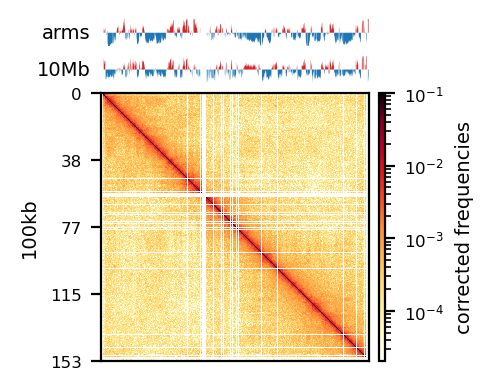
\includegraphics[width=2.57292in,height=2.03125in]{index_files/figure-latex/..-notebooks-07_various_plotting-fig-rs100-recpe-pe-output-1.png}

}

\subcaption{\label{fig-rs100-recpe-pe-1}recPE RS 100kb full chrX}

\end{minipage}%
%
\begin{minipage}{0.46\linewidth}

\centering{

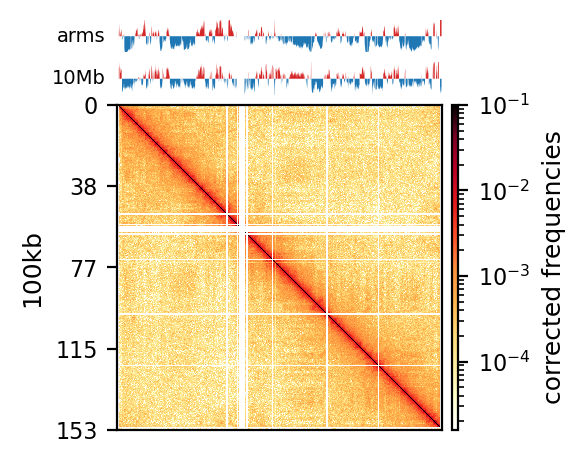
\includegraphics[width=2.57292in,height=2.03125in]{index_files/figure-latex/..-notebooks-07_various_plotting-fig-rs100-recpe-pe-output-2.png}

}

\subcaption{\label{fig-rs100-recpe-pe-2}PE RS 100kb full chrX}

\end{minipage}%
%
\begin{minipage}{0.05\linewidth}
~\end{minipage}%
\newline
\begin{minipage}{0.05\linewidth}
~\end{minipage}%
%
\begin{minipage}{0.46\linewidth}

\centering{

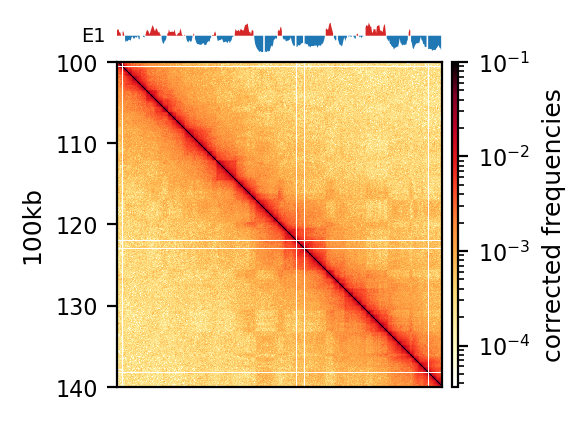
\includegraphics[width=2.57292in,height=2.09375in]{index_files/figure-latex/..-notebooks-07_various_plotting-fig-rs100-recpe-pe-output-3.png}

}

\subcaption{\label{fig-rs100-recpe-pe-3}recPE RS 100kb chrX:70Mb-78Mb}

\end{minipage}%
%
\begin{minipage}{0.46\linewidth}

\centering{

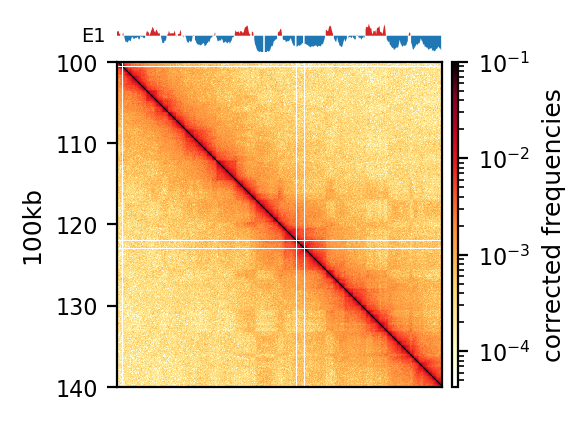
\includegraphics[width=2.57292in,height=2.09375in]{index_files/figure-latex/..-notebooks-07_various_plotting-fig-rs100-recpe-pe-output-4.png}

}

\subcaption{\label{fig-rs100-recpe-pe-4}PE RS 100kb chrX:70Mb-78Mb}

\end{minipage}%
%
\begin{minipage}{0.05\linewidth}
~\end{minipage}%

\caption{\label{fig-rs100-recpe-pe}Round Spermatid (RS) at 100kb,
comparing the impact of parsing parameters}

\end{figure}%

To emphasize the findings, the sets of A-compartments were compared
between the two parsing runs, showing almost identical compartment
calls. Additionally, the set difference was 8 bins between PE and recPE
for round spermatid 100kb and 5 bins for fibroblast for \emph{arms}
viewframe (Figure~\ref{fig-rs-fb-100-pe-recpe-intervals}; a+b,
respectively). We observe a high number of differences around 76Mb for
the refined compartments (10Mb) of round spermatid, which is consistent
with the sign-flip of E1 values discussed earlier. Anything else would
be surprising, as it is the same data, but visualized in a different
way.

\begin{figure}

\begin{minipage}{0.10\linewidth}
~\end{minipage}%
%
\begin{minipage}{0.40\linewidth}

\centering{

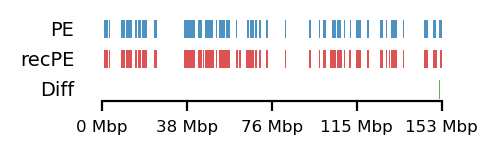
\includegraphics[width=2.59375in,height=0.80208in]{index_files/figure-latex/..-notebooks-07_various_plotting-fig-rs-fb-100-pe-recpe-intervals-output-1.png}

}

\subcaption{\label{fig-rs-fb-100-pe-recpe-intervals-1}RS: arms}

\end{minipage}%
%
\begin{minipage}{0.40\linewidth}

\centering{

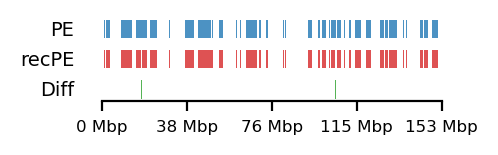
\includegraphics[width=2.59375in,height=0.80208in]{index_files/figure-latex/..-notebooks-07_various_plotting-fig-rs-fb-100-pe-recpe-intervals-output-2.png}

}

\subcaption{\label{fig-rs-fb-100-pe-recpe-intervals-2}Fib: arms}

\end{minipage}%
%
\begin{minipage}{0.10\linewidth}
~\end{minipage}%
\newline
\begin{minipage}{0.10\linewidth}
~\end{minipage}%
%
\begin{minipage}{0.40\linewidth}

\centering{

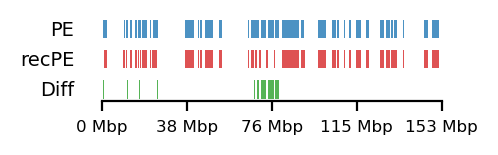
\includegraphics[width=2.59375in,height=0.80208in]{index_files/figure-latex/..-notebooks-07_various_plotting-fig-rs-fb-100-pe-recpe-intervals-output-3.png}

}

\subcaption{\label{fig-rs-fb-100-pe-recpe-intervals-3}RS: 10Mb}

\end{minipage}%
%
\begin{minipage}{0.40\linewidth}

\centering{

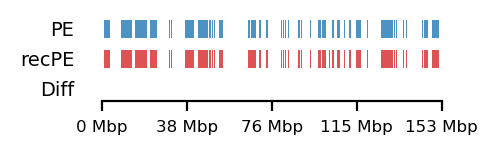
\includegraphics[width=2.59375in,height=0.80208in]{index_files/figure-latex/..-notebooks-07_various_plotting-fig-rs-fb-100-pe-recpe-intervals-output-4.png}

}

\subcaption{\label{fig-rs-fb-100-pe-recpe-intervals-4}Fib: 10Mb}

\end{minipage}%
%
\begin{minipage}{0.10\linewidth}
~\end{minipage}%

\caption{\label{fig-rs-fb-100-pe-recpe-intervals}Round Spermatid (RS)
and Fibroblast (Fb) at 100kb, comparing the impact of parsing parameters
on A-compartment calling at different viewframes; \emph{arms},
\emph{10Mb}. PE: initial parse (masking complex walks); recPE:
recommended parse (reporting the 5'most unique alignment of a complex
walk).}

\end{figure}%

The observed difference between the sets can for our data be attributed
to chance, but we cannot draw general conclusions about the parameters
in general. I argue that the quality and size of the Hi-C library will
influence sensitive to parsing parameters. In that case, the most
flexible approach is still to follow the recommendations from
\texttt{cooler} to report more pairs as valid contacts, and then create
coolers with different \emph{mapq} filters if issues are encountered.

\subsection{Compartment Edges (transition
zones)}\label{compartment-edges-transition-zones}

We compare how the ECH90 regions fit when queried on top of the
A-compartments and equivalently for the edges, for fibroblasts and round
spermatids at 100kb resolution. When queried against the edges in stead,
the the total set size is reduced to less than 50\%. Interestingly, some
of the intersections between A-compartments and ECH90 remain, and new
ones appear as we move to the outside edge of the compartment
(Figure~\ref{fig-comps-edges-ech}). This indicates that most, but not
all, of the intersection between ECH90 regions and the A-compartments
are within 100kb of the compartment edge, and additional overlap is
gained if we define a transition zone on the outside of the edge as
well. To visualize this (outside) edge enrichment, we find the set
difference of the ECH-intersection to compartments and edges,
respectively (Figure~\ref{fig-edge-enrichment}), thus removing all the
`inside' edges. We observe that in almost all of the of the regions of
\(ECH \cap Comp\) are accompanied by an edge also intersecting ECH
(\(ECH \cap Edge\)), localized where the \emph{Diff} track aligns
(within 100kb) with both \(CompInt\) and \(EdgeInt\).

\begin{figure}

\begin{minipage}{0.10\linewidth}
~\end{minipage}%
%
\begin{minipage}{0.40\linewidth}

\centering{

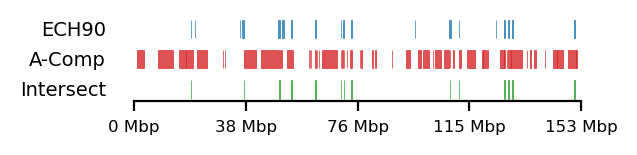
\includegraphics[width=2.58333in,height=0.80208in]{index_files/figure-latex/..-notebooks-07_various_plotting-fig-comps-edges-ech-output-1.png}

}

\subcaption{\label{fig-comps-edges-ech-1}Fibroblast A-compartments}

\end{minipage}%
%
\begin{minipage}{0.40\linewidth}

\centering{

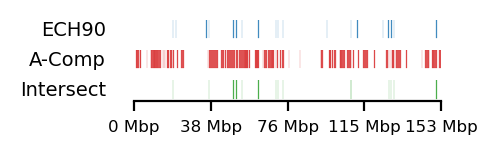
\includegraphics[width=2.58333in,height=0.80208in]{index_files/figure-latex/..-notebooks-07_various_plotting-fig-comps-edges-ech-output-2.png}

}

\subcaption{\label{fig-comps-edges-ech-2}Round Spermatid A-compartments}

\end{minipage}%
%
\begin{minipage}{0.10\linewidth}
~\end{minipage}%
\newline
\begin{minipage}{0.10\linewidth}
~\end{minipage}%
%
\begin{minipage}{0.40\linewidth}

\centering{

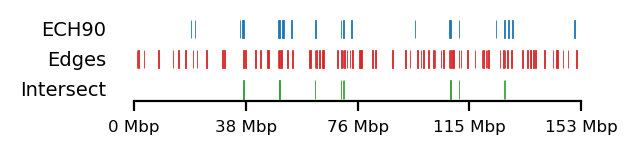
\includegraphics[width=2.58333in,height=0.80208in]{index_files/figure-latex/..-notebooks-07_various_plotting-fig-comps-edges-ech-output-3.png}

}

\subcaption{\label{fig-comps-edges-ech-3}Fibroblast edges}

\end{minipage}%
%
\begin{minipage}{0.40\linewidth}

\centering{

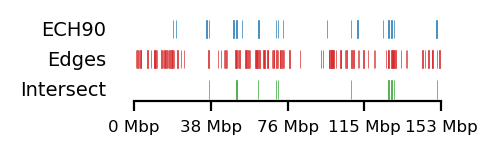
\includegraphics[width=2.58333in,height=0.80208in]{index_files/figure-latex/..-notebooks-07_various_plotting-fig-comps-edges-ech-output-4.png}

}

\subcaption{\label{fig-comps-edges-ech-4}Round Spermatid edges}

\end{minipage}%
%
\begin{minipage}{0.10\linewidth}
~\end{minipage}%

\caption{\label{fig-comps-edges-ech}Visual representation of the genomic
intervals of ECH90, A-compartments (a+b), edges (c+d), and their
intersections. Shown fibroblast (a+c) and round spermatid (b+d) at 100kb
resolution and arms viewframe.}

\end{figure}%

\begin{figure}

\begin{minipage}{0.50\linewidth}

\centering{

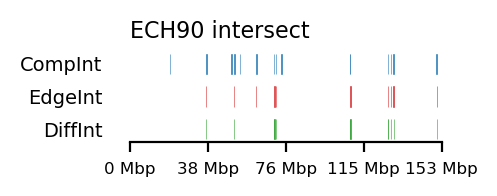
\includegraphics[width=2.58333in,height=1.02083in]{index_files/figure-latex/..-notebooks-07_various_plotting-fig-edge-enrichment-output-1.png}

}

\subcaption{\label{fig-edge-enrichment-1}Round Spermatid}

\end{minipage}%
%
\begin{minipage}{0.50\linewidth}

\centering{

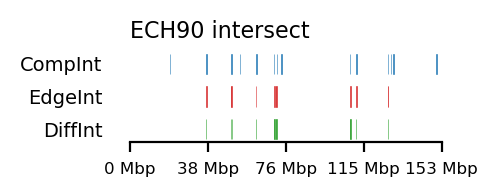
\includegraphics[width=2.58333in,height=1.02083in]{index_files/figure-latex/..-notebooks-07_various_plotting-fig-edge-enrichment-output-2.png}

}

\subcaption{\label{fig-edge-enrichment-2}Fibroblast}

\end{minipage}%

\caption{\label{fig-edge-enrichment}Visual representation of the
enrichment of edges in the intersection of ECH90 and A-compartments.
Shown round spermatid (a) and fibroblast (b) at 100kb resolution and
arms viewframe. Note that the edge-regions are too small to be
distinguished visually from the compartment on the graph, making it look
like they overlap, even though the difference is reported.}

\end{figure}%

We apply both proximity test and Jaccard test, to see how well the
results could occur by chance (Figure~\ref{fig-proximity-jaccard-bar}).
For completeness, the tests are included for all cell types, but we only
use 100kb resolution arms viewframe. We observe that both fibroblast and
round spermatid have \(p < 0.05\) for both tests, meaning the two cell
type have both more intersection with ECH regions than expected by
chance (Jaccard) \emph{and} the non-overlapping intervals are more
proximal to compartment edges than expected by chance (proximity test).
I argue that a significant Jaccard statistic should be interpreted as a
significant amount of overlap between the two sets, i.e.~compartment
edges and ECH90 regions, and the proximity test (when performed on the
edges) gives us information about the potential of expanding the
transition window. That is, if the non-overlapping regions are
\emph{very} proximal, a larger (or shifted) to only capture the 200kb
region outside of the edge.

\begin{figure}[H]

\centering{

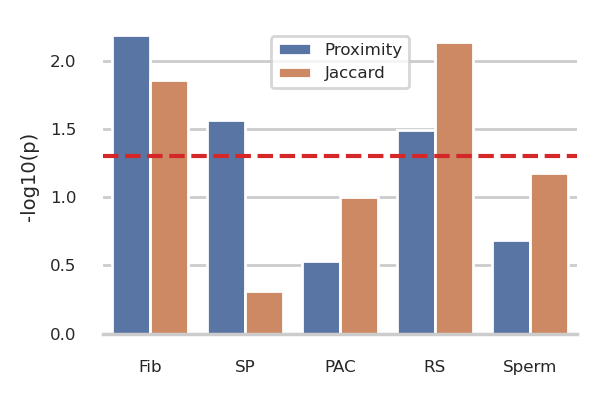
\includegraphics[width=3.10417in,height=2.05208in]{index_files/figure-latex/..-notebooks-06_rec_genomicintervals-fig-proximity-jaccard-bar-output-1.png}

}

\caption{\label{fig-proximity-jaccard-bar}Proximity and Jaccard index
p-values for ECH90 regions on compartment edges for all cell types at
100kb resolution at arms view \(p=0.05\) is marked as a red line.}

\end{figure}%

\newpage{}

\chapter{Discussion}\label{discussion}

Here is the discussion

\chapter*{Bibliography}\label{bibliography}
\addcontentsline{toc}{chapter}{Bibliography}

\begingroup
\raggedright

\renewcommand{\bibsection}{}
\bibliography{../references.bib}

\endgroup


\backmatter



\end{document}
